\clearpage
\section{多元函数微分学}

\subsection{复习要点} \par

\subsubsection{研究多元函数的一般原则}\par

研究多元函数（以二元函数为例）如同探索一片山区.
在地图上，经度和纬度可以分别视为$x$坐标和$y$坐标，而每一个经纬度都对应于一个海拔高度.
因此，海拔高度$z$显然是关于$x$和$y$的二元函数，可以记为$z = f(x,y)$.
这样一来，整片山区本身就是就是$f(x,y)$的函数图像.

这个比喻适用于一切关于二元函数的讨论.
在讲义中我们会时常借用这个比喻来帮助理解.\par
对于二元函数的研究，首先应该分清两个层次的视角：
“路径视角”和“全面视角”.
假设有一个探险者要翻越整片山区，他只能沿着某条固定的路径前进.
在这条路径上，探险者所经历的海拔高度可以视为关于前进距离的一元函数，而我们已经学习过一元函数的微积分，就可以对海拔高度的变化形势加以研究了.
这就是从“路径”层面获得的观点.

上述方法存在两个问题. 其一，探险者虽然能认识到自己路线上的地形状况，但对自己路线之外的地形还是一无所知的.
想要真正了解整片区域内的地形，必须沿无数条覆盖整片区域的不同的路径来进行考察，这显然是无法完成的.
其二，会有“横看成岭侧成峰”的情况出现，
即对于同一个问题，沿着不同的路径来研究可能得到不同的结论.
综上所述，我们不能局限于单一路径上的观点，
应该要把不同路径的情况综合起来考量，最终提出一些不依赖于路径选取的结论；
或者干脆规定一些与路径无关的性质，以便于研究. 这就是“全面”的视角.\par
最后，对于教材$6.1$节中介绍的概念，尤其是$\mathbb{R}^n$中\textbf{开集}、\textbf{边界}、\textbf{闭集}与\textbf{连通性}的定义，同学们至少需要脸熟一下.
在高数课程中，这些概念主要是用于描述定义域的，仅从直观上理解亦可（如$\mathbb{R}^2$中的开集就是不包含边界的平面区域）.

\subsubsection{二元函数的（全面）极限与累次极限} \par

考虑二元函数$z = f(x,y)$. 从路径观点来看，当我们选定了一条趋向目标点$P_0(x_0,y_0)$的路径之后，就可以在一元函数的意义上讨论函数$f$在$P$点处的极限.
例如，若选择沿直线$y=x$从右侧趋向$(0,0)$，问题就变成了求一元函数$F(x) = f(x,x)$在$x = 0$处的右极限.
然而，这样计算的结果可能与路径的选取的有关.
因此在讨论$n$元函数的极限时，（实际上可以通过定义证明）我们有以下的要求:\par \vspace{1em}

\textbf{$n$元函数极限存在的充要条件}~~\textit{$n$元函数在点$P_0$处的极限存在，当且仅当点$P$沿任意路径趋向$P_0$时的极限存在且相等.}
\textit{（对于一元函数，上述条件就是指“左右极限存在且相等”）} \vspace{0.5em}

路径的任意性表明，多元函数的极限是一个“全面视角”下的概念.
反过来，可以给出判断$n$元函数极限不存在的准则. 这在做题时常用： \vspace{0.5em}

\textbf{$n$元函数极限不存在的判断准则}~~\textit{若以下两条其中之一成立，则可以判断$n$元函数在点$P_0$处的极限不存在：}\par
\textit{(1)~~点$P$沿某条路径趋向$P_0$时的极限不存在；}

\textit{(2)~~点$P$沿两条不同的路径趋向$P_0$时的极限值不同.} \vspace{0.5em}

以上关于$n$元函数极限的叙述已经充分了. 需要额外提醒是，路径不是只能取直线的.
有的函数沿一切直线路径趋向点$P_0$的极限都存在且相等，然而沿某条曲线路径取得的极限值与之不同，导致函数的极限不存在.
这种情况教材中已经举了例子.\par
教材中$6.2.3$还补充了另一种取极限的方法，即可以依次取$x \to x_0$和$y \to y_0$（或先取$y \to y_0$再取$x \to x_0$）.
用这种方法取到的极限称为\textbf{累次极限}. 教材中强调，累次极限与之前所定义的极限（也称为\textbf{全面极限}）是完全不同的两个概念，具体表现为：
全面极限存在不意味着累次极限存在，两种累次极限存在且相等也不能保证全面极限存在.
一些同学可能对前半句话心存疑问：“累次极限难道不就是沿$x = x_0$（或$y = y_0$）这样一种特殊路径取得的极限吗？”
这种理解是错误的. 拿教材中所举的例子来说：
\begin{eq1}
    \setstretch{1.25}
    f(x,y) =
    \begin{cases}
        (x+y) \sin \frac{1}{x} &\quad x \ne 0 \\[4pt]
        0 &\quad x = 0
    \end{cases}
\end{eq1} \setstcolor{1.75}

书中指出它的累次极限$\lim\limits_{y \to 0} \limx0 f(x,y)$不存在.
但是沿路径$x=0$的极限显然为$0$.
这也等于它的全面极限.
可见，不能将累次极限理解为一种沿特殊路径的极限.
累次极限与全面极限没有必然联系，因此在做题的过程中可以利用特殊路径帮助判断极限是否存在，
但是\textbf{不要使用累次极限}.\par \vspace{1em}

如果要证明一个二元函数在某点处极限存在，用上面的方法是行不通的，因为我们不可能遍历所有的路径.
用$\epsilon - \delta$定义来证明也比较复杂（一般不会这样考）.
这时我们一般要用极限的运算法则与基本性质.
与第一章类似，我们在讲义中列出同学们应该掌握的定理，但不赘述其内容，只做一些评注：\par \vspace{1em}

(1)~~\textbf{极限的四则运算}~~具体内容类似于一元函数. 以极限相加为例，要注意：两个函数之和的极限如果要拆成两个函数极限之和，前提是这两个函数的极限分别存在.\par
(2)~~\textbf{极限不等式}~~具体内容类似于一元函数. 进一步可以得到极限的保号性性质.\par
(3)~~\textbf{夹逼定理}~~最重要. 常用于证明“极限为$0$”乘以“有界”的极限为$0$.\par
(4)~~\textbf{复合函数的极限}~~用一句话概括：无论内外层函数是一元函数还是二元函数，只要所有内外层函数的极限都存在，那么复合之后的极限存在.\par

\subsubsection{知识主线1——连续、可微、与可偏导的关系} \par
从本小节开始，我们将带领大家以一个与教材略有不同的顺序来梳理第六章的知识点.
希望可以帮助大家理解和记忆.

对二元函数的研究也遵循一条“\textbf{极限—连续—可微}”的主线，
相关概念的定义方式和互推关系可以完全类比一元函数的情形.
我们强调，二元函数“极限”、“连续”和“可微”这三个概念都是不选取路径的，也就是我们所谓的“全面视角”下的观点.
而像“偏导数”、“方向导数”、“链式法则”这些在多元函数中特有的概念，实质都是在特定的路径和方向上来研究多元函数，也就是“路径视角”.
现在，让我们先忘掉“偏导数”等概念，先将“极限—连续—可微”这个主线解释清楚.\par

如果二元函数在某点处的极限等于该点的函数值，就说二元函数在该点处\textbf{连续}.
回忆第一章中学习的一元连续函数在闭区间上的性质，并进行类比：
二元连续函数在\textbf{闭区域}中也有\textbf{有界定理}、\textbf{最值定理}和\textbf{介值定理}这“三剑客”.\par
二元函数\textbf{可微}的定义，道理与一元函数完全相同，只是具体表达式有一点差异.
二元函数$z = f(x,y)$在$(x_0,y_0)$处可微是指，\textbf{全增量}$\Delta z$可以表示为\textbf{线性主要部分}$A \Delta x + B \Delta y$
加上一个高阶无穷小量$o(\rho)$. 其中，$\rho$是点$(x,y)$到$(x_0,y_0)$之间的距离.
\textbf{二元函数连续不一定可微，可微一定连续}，这一点也与一元函数相同.
所以，如果不考虑高阶微分的话，“可微”就是对一个二元函数最高的要求了.\par
请注意，北大版教材在讨论多元函数时没有“可导”这个概念，我们也建议同学们不要使用“可导”来代替“可微”，最好“可导”这两个字连用都不要用.
别的书中出现“可导”二字时，一般是指“可偏导”，所以如果一定要说，多元函数中的“可导”并不等价于“可微”.\vspace{1em}

接下来，我们可以解锁“偏导数”这个概念了.
众所周知，对$x$求偏导数，其实就是将$y$视为常数，把$f(x,y)$关于$x$的一元函数来求导.
同学们可能觉得，偏导数的概念比微分理解起来更容易，就把偏导数作为一个核心概念来理解了.
但事实上，偏导数这个概念与“极限—连续—可微”的主线是格格不入的.
具体表现在：\textbf{二元函数连续不一定可偏导，而且可偏导也不一定连续，甚至不一定存在极限.}
对于后半句话，可以举出下面这个简单而深刻的反例：
\begin{eq1}
    \setstcolor{1.25}
    f(x,y)=
    \begin{cases}
        -100 &\quad x = 0\text{~或~} y=0 \\[-4pt]
        0 &\quad x\text{、}y \ne 0
    \end{cases}
\end{eq1} \setstretch{1.75}

这个函数相当于在平地上一横一竖挖了两道$100$米深的沟.
对$x$或$y$求偏导，相当于沿着深沟求导，显然偏导数都是$0$.
但是$f(x,y)$在$(0,0)$处连极限都不存在，更不用说连续或者可微了.
如果大家愿意，可以用这种“挖沟法”构造在一点处所有方向导数都存在，但是不连续的函数.
这个例子形象地表明，“路径视角”下的偏导数概念，与“全面视角”下的概念之间有不可逾越的“鸿沟”.
沿着一条沟求出的导数，对描述函数在一点邻域内的全面性质几乎毫无作用.\par
说到这里，同学们应该能猜到：\textbf{二元函数可偏导不一定可微}，而\textbf{二元函数可微则一定可偏导}.
后半句话涉及到“导数”与“微分”的关系——“线性主要部分”中的$A$和$B$实际上分别就是$\frac{\partial z}{\partial x}$和$\frac{\partial z}{\partial y}$.\par
此外，教材中一个定理指出，用一些“赖皮”的方法也能利用偏导数保证函数的可微性：\par \vspace{0.5em}

\textbf{可微的充分条件}~~\textit{若函数$f(x,y)$的偏导数$f_{x}(x,y)$与$f_{y}(x,y)$在点$(x_0,y_0)$的某个邻域内存在，
并且这两个偏导数在点$(x_0,y_0)$处连续，则$z = f(x,y)$在点$(x_0,y_0)$处可微.}\par \vspace{0.5em}

以上关于偏导数的条件之所以能成为可微的充分条件，
是因为对整个“邻域内”的所有偏导数提出了连续的要求.
形象地说，是分别沿着$x$轴和$y$轴的方向把整片邻域全部犁了一遍，从而事实上全面地覆盖到了整片区域.\par
不过，这个定理也有有趣之处.
按照讲义开篇的“爬山”比喻，我们的“探险者”必须走遍所有可能的路径，才能获得对地形的全面理解.
但是在这个定理中，这位“探险者”事实上只尝试了所有横向和纵向的路径，就得出了可微的结论.
这里甚至都没有尝试其他方向的直线路径，更不用说曲线路径了.

\subsubsection{*知识主线2——偏导数、方向导数、复合函数求导、梯度} \par
在第2条知识主线中，我们来探讨与路径有关的一些概念.
学会这些知识点本身并不难，但是真正理解它们需要更深刻地思考.
如果同学们认为自己对标题中相关概念的掌握已经足够应对考试，
可以跳过本小节.

讲义前文和教材中都提及，
偏导数是沿$x$轴和$y$轴这两个特殊方向的导数.
但是这种“特殊性”是坐标系所导致的.
不妨脱离坐标系来这样考虑：对于给定曲面上的任意一点，如果该点可微，我们就可以过这个点作曲面的切平面.
另外，也可以过该点作无数条不同方向的切线，这些切线全在切平面上.
与一元函数求导类似，沿某个方向求导数的几何意义就是求切线的斜率.
但是，如果没有指定坐标系，不同方向的切线都是“平权”的，没有任何一个方向是所谓的“特殊”方向.
一旦指定了$x$轴和$y$轴的方向，并按这个坐标系写出曲面的方程，则这两个方向的导数就变得比较好求，这就是偏导数.\par

如果把上面所说的“切线”改为“切向量”（图1），那么可以想到：
由于过某点的切向量都共面于切平面，那么作为平面向量，它们应该服从平面向量分解定理.
也就是说，沿任意方向的切向量$\bm{T}$都可以分解到两个特殊的方向上，写成两个基向量（$\bm{e}_x$和$\bm{e}_y$）的“线性组合”.
为了计算方便，这两个“特殊的方向”就取为$x$轴方向和$y$轴方向，两个基向量$\bm{e}_x$和$\bm{e}_y$的斜率分别就是两个偏导数.
所谓的\textbf{方向导数}，其实就是沿其他方向的切向量的斜率.
感兴趣的同学可以尝试：若把任意切向量$\bm{T}$表示成$\bm{e}_x$和$\bm{e}_y$的“线性组合”，并将任意切向量的斜率用基向量的斜率表示出来，也可以推导出方向导数公式：\par

\begin{figure}[H]
    \centering
    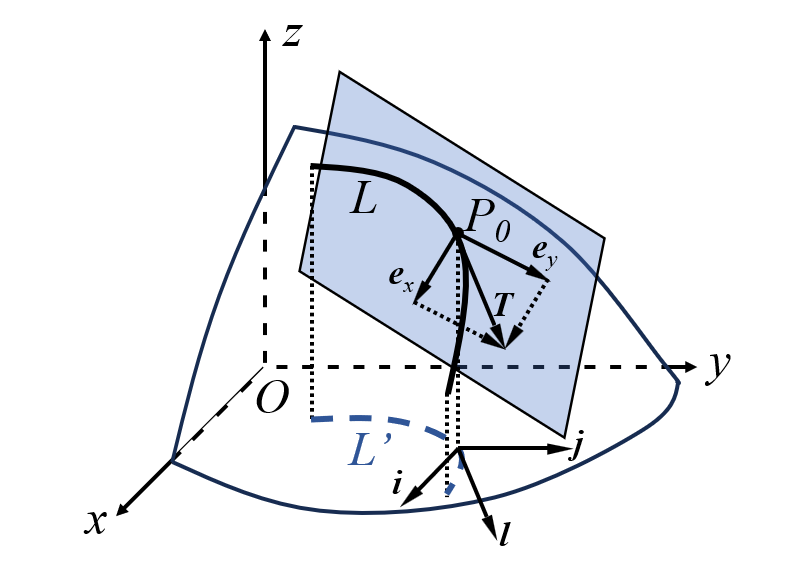
\includegraphics[width=0.6\textwidth]{Fig1.png}
    \caption{方向导数、复合函数求导与切向量}
\end{figure}

设$z = f(x,y)$在$P_0(x_0,y_0)$处可微，则沿向量$\bm{l}$的方向导数为：
$$
\setlength\abovedisplayskip{12pt}
\setlength\belowdisplayskip{12pt}
\left. \frac{\partial f}{\partial \bm{l}} \right|_{P_{0}} = f_x(x_0,y_0)\cos \alpha + f_y(x_0,y_0) \cos \beta
$$\par
将这个公式与复合函数求导进行比较：设二元函数$z=f(x,y)$中，$x$与$y$分别都是关于$t$的函数，记作$x=x(t)$和$y=y(t)$. 则有：
$$
\setlength\abovedisplayskip{12pt}
    \setlength\belowdisplayskip{12pt}
\frac{\d f}{\d t} = f_x (x_0,y_0) \frac{\d x}{\d t} + f_y (x_0,y_0) \frac{\d y}{\d t}
$$

可以发现两个公式是十分类似的. 甚至如果“恰好”让$\frac{\d x}{\d t}$和$\frac{\d y}{\d t}$分别等于$\cos \alpha$和$\cos \beta$，
那么$\frac{\d f}{\d t}$就可以视作一个方向导数了.
但是这个看法的具体意义是什么呢？
我们借助爬山的比喻来进一步解释.\par
假设有一位探险者在曲面上前进，将他的运动轨迹（图1中位于曲面内的曲线$L$）描绘记录下来并投影到$xOy$平面上，
得到的平面曲线（图1中蓝色虚线所代表的曲线$L'$）可以用一组参数方程来描述.
其实，刚才做复合函数求导时所给出的函数$x = x(t)$和$y = y(t)$的意义，就是这里的平面曲线的参数方程.
根据我们第五章对曲线参数方程的讨论，如果把变量$t$看成时间的话，那么参数方程不仅给出了探险者（在$xOy$投影上）
的行进路线，而且$\frac{\d x}{\d t}$和$\frac{\d y}{\d t}$还能表示他水平移动的速度.
那么复合函数求导$\frac{\d f}{\d t}$的意义就是：\textbf{探险者按参数方程$x(t)$和$y(t)$所规定的速率运动时，其海拔高度$z$关于时间的变化率}.
而按照之前关于切平面和向量分解的讨论，我们可以说：爬山引起的海拔变化的趋势，可以分解为沿$x$轴的“坡度”和沿$y$轴的“坡度”两部分.
这就是对“全微分”的解释.\par
更进一步，$\frac{\d f}{\d t}$在任一时刻的取值实际上与整条路径关联不大，仅与探险者当前所处的位置以及速度有关.
而速度的方向其实就是曲线的切线方向.
从这个意义上讲，求全导数$\frac{\d f}{\d t}$其实也只是对$z = f(x,y)$沿特定方向求导，只不过这个“特定方向”是由
复合函数的内层函数（视作曲线的参数方程）所决定的.
然而，正如前面所讨论的，“海拔高度随时间的变化速率”与“探险者”的行走速度有关；
但是如果只谈及“坡度”、“切线斜率”等概念，则只是对地形的客观描述，与行走速度无关.
如果要通过“探险者”的运动来反映客观的“坡度”，最好的方法是让他（在$xOy$投影上）以单位速率运动.
这就是说：
$$
\setlength\abovedisplayskip{12pt}
    \setlength\belowdisplayskip{12pt}
|\bm{v}| = \sqrt{\left(\frac{\d x}{\d t}  \right)^2 + \left(\frac{\d y}{\d t}  \right)^2} = 1
$$
\setstretch{1.75}

$\frac{\d x}{\d t}$和$\frac{\d y}{\d t}$有平方和的关系，意味着它们同时也可以视为$L'$在$P_0$处的切向量$\bm{l}$的方向余弦.
这时，$\frac{\d f}{\d t}$和$\frac{\partial f}{\partial \bm{l}}$没有区别了.

本节的最后，我们简要讲解一下\textbf{梯度}的概念.
二元函数中谈及的梯度是$xOy$平面上的向量，等于$(f_x,f_y)$.
其物理意义是：\textbf{梯度方向是上山最“费力”的方向，负梯度方向是下山最“省力”的方向}.
沿梯度方向的方向导数，即该方向上的“坡度”，等于梯度的模长.
引入梯度这一概念的意义不仅在于研究怎么下山最快（可能是用滚的），其物理意义也是十分深刻的——
\textbf{任何保守势场的负梯度都是相应的保守力}.
以下两个更加具体的例子可能唤醒同学们的高中记忆：

(1)~~电势的负梯度是电场强度（例\ref{ex:ch06-12}）；

(2)~~大气压的负梯度是气压梯度力（大气环流的动力之一）.

\subsubsection{关于求导法则的补充说明}

求导（尤其是复合函数的导数）本身没有特别的技巧，同学们多加练习即可.
但是在多元函数中各种求导符号的混乱经常会造成迷惑.
因此，有必要花些篇幅来解释.

最重要的是偏微分/偏导数（用$\partial$表示）和全微分/全导数（用$\d$表示）的区别.
教材上的区分很明确：
如果是多元函数求导，就用偏导数表示；
如果是一元函数求导，就用全导数来表示.
例如，上节中提到的复合函数$f\left( x(t),y(t) \right)$，
虽然看起来是二元函数，
但是究其根本，$x$和$y$都是$t$的函数，所以整个函数可以看成关于$t$的一元函数，因此$f$对$t$求导就应该写成$\frac{\d f}{\d t}$.
但如果$x$和$y$都是关于$t$和$u$两个变量的二元函数$x(t,u)$和$y(t,u)$，
那么整个函数$f$亦可看成关于$u$和$v$的二元函数，
这时再要写$f$对$t$的导数，
就应写成$\frac{\partial f}{\partial t}$了.
可见，在复合函数求导的情况下，我们必须十分关注内外层变量之间的函数关系.
一般情况下，一个函数对一个特定的变量求导，
只能是偏导数或全导数其中之一.

我们请同学们注意这个细节，不仅是为了书写规范，更重要的是为了辨别一些“模棱两可”的情况.
实际上在隐函数相关的问题里经常会遇到这样的情况. 考虑以下的隐函数方程：
$$
\setlength\abovedisplayskip{6pt}
    \setlength\belowdisplayskip{6pt}
f(x,y) = 0
$$

现在要求函数$f$对$x$的导数，应该怎么做？
正确答案是“不知道”，因为我没有说是求偏导数还是全导数，而这两者是有区别的！——
(1)~如果要求对$x$求偏导数，说明是将等号左边正常理解为了二元函数，求导结果就是$\frac{\partial f}{\partial x}$.
(2)~如果要求对$x$求全导数，说明是将等号左边理解为了一元函数——但是为什么能这样理解？
我们知道，在条件合适的情况下，上面的隐函数方程可以确定一个$y$关于$x$的一元函数，
那么$f(x,y)$自然也可以看成关于$x$的一元函数. 因此有：
$$
\setlength\abovedisplayskip{12pt}
    \setlength\belowdisplayskip{12pt}
\frac{\d f}{\d x} = \frac{\partial f}{\partial x} + \frac{\partial f}{\partial y} \cdot \frac{\d y}{\d x}
$$

上面这个式子很好地反映了偏导数与全导数的区别.
到此为止，同学们可能觉得讨论已经十分完全了.
但是且慢！
我们再看一个从教材上取来的例子：
$$
\setlength\abovedisplayskip{6pt}
    \setlength\belowdisplayskip{6pt}
F\left(x,y,u(x,y),v(x,y)\right)
$$\par
这个例子出现在6.8节的例5之前的一段正文中.
它说，求函数$F$关于变量$x$的偏导数，结果是这样：
$$
\setlength\abovedisplayskip{6pt}
    \setlength\belowdisplayskip{6pt}
\frac{\partial F}{\partial x} +
\frac{\partial F}{\partial u} \cdot \frac{\partial u}{\partial x}
+\frac{\partial F}{\partial v} \cdot \frac{\partial v}{\partial x}
$$\par
这是可以理解的，因为既然$u$和$v$都是关于$(x,y)$的二元函数，那么$F$自然也可以看成关于$(x,y)$的二元函数，
这样得到的求导结果就是上面这样了.
但是离奇的是，
上面这个式子中竟然又出现了$\frac{\partial F}{\partial x}$，
这也是“$F$对$x$的偏导数”，
但它的意义竟然与上面说的又有所不同.
因为按照链式法则，这里的$\frac{\partial F}{\partial x}$
是指将$F$视作一个四元函数，
求其第一分量的偏导数.
而在其第一分量位置的不是别的，正是$x$自己，
因此这个四元函数的偏导数也被记成了$\frac{\partial F}{\partial x}$.
这就已经造成记号上的混乱了.

有了上面的讨论，相信同学们已经能正确理解偏导数记号中的bug.
同学们自己在书写的时候，如果要避免这个bug，
推荐另一种常用的偏导数记号：
以多元函数$F(x,y,u,v)$为例，分别用$F_1,F_2,F_3,F_4$表示$F$对第一、二、三、四分量求偏导.
这样做的好处是，无论括号内四个“输入槽”里的字母如何变动，数字角标所代表的意义是不会变的.
而$f_x$或$\frac{\partial F}{\partial x}$用于指代对具体的变量$x$求偏导.
这样一来，$F\left(x,y,u(x,y),v(x,y)\right)$
对$x$求偏导就可以写成：
$$
\setlength\abovedisplayskip{6pt}
    \setlength\belowdisplayskip{6pt}
\frac{\partial F}{\partial x} =
F_1 + F_3 \cdot u_x + F_4 \cdot v_x
$$\par
最后再说明一个问题.
对于二元函数$z = f(x,y)$，
我们一般把$\frac{\partial z}{\partial x}$和$\frac{\partial f}{\partial x}$看作是完全相同的东西.
但其实二者的意义是有所不同的：前者是对“变量”求导，后者是对“函数”求导.
二者的区别会造成一个问题：同一个变量可以用不同的函数关系来描述，而不同的函数关系中除了具有不同的自变量以外，也可以共用一些相同的自变量.
设多元函数$z = g_1(x,\cdots)$和$z = g_2(x,\cdots)$中都含有自变量$x$，
那么$\frac{\partial g_1}{\partial x}$与
$\frac{\partial g_2}{\partial x}$很有可能是不同的，
但是如果都写成$\frac{\partial z}{\partial x}$就无从区分了.
这个细节曾经出在了期末考题中（例\ref{ex:ch06-15}），请同学们关注.

\subsubsection{隐函数存在定理（极简版复习导引）} \par
教材6.8节介绍了隐函数存在定理和逆映射存在定理，以及多种不同的情况.
这些都需要完全掌握.
但是绝不能一条条去背诵.
只要学会对方程求偏导来求解隐函数的偏导数的方法，就可以一通百通了.
见书上6.8节例2和关于方程组（6.7）的叙述.
因为在对方程求完偏导数之后，实际上就转化成了求解线性方程组的问题.
而书上最复杂的情况也不过是两个方程的情况，最终只需要解二元一次方程组.
大致来说，线性方程（组）有\textbf{唯一解}的条件就是隐函数唯一存在的条件.
知道这一点后，再去复习每种不同情况下隐函数存在定理的条件，
相信大家能明白不同的情况没有任何实质区别.\par
考试时，既有可能要求“证明隐函数唯一存在”，也有可能要求“计算隐函数的偏导数”.
注意这是两种不同的题型.
如果是前者，必须一一验证隐函数存在定理的所有条件，将它们清楚地列在答题纸上，但不一定要具体求出隐函数的偏导数；
如果是后者，只需用6.8节例2中的三种方法之一直接开始计算即可.
其中推荐掌握第三种方法，即全微分法.
因为在只有一条方程而有多个自变量的情况下，取全微分可以一次性获得隐函数的所有偏导数，
这样就无需背公式或者计算多次.\par

\subsubsection{知识主线3——高阶微分、二元函数的泰勒公式、极值问题} \par
二元函数的高阶微分的表达式如下：
$$
\setlength\abovedisplayskip{6pt}
\setlength\belowdisplayskip{6pt}
\d ^n f = \left( \d x \frac{\partial}{\partial x} + \d y \frac{\partial}{\partial y} \right)^n f
$$\par
具体计算时，需将括号按照牛顿二项式展开.
一般的高阶微分主要应用是计算\textbf{二元函数的泰勒公式}.
这方面的要求不如一元函数的泰勒公式那么高，
只需要通过求偏导数算出高阶微分，代入泰勒公式即可.
这里我们展示$f(x,y)$在$(x_0,y_0)$处的二阶的泰勒多项式（已将二阶微分展开），因为考试一般只考到这个程度：
\begin{eq1}
    f(x,y) &\sim
    f(x_0,y_0) + f_x(x_0,y_0)\Delta x + f_y(x_0,y_0)\Delta y \\
    &+ \frac{1}{2} \left[ f_{xx}(x_0,y_0)(\Delta x)^2 + 2f_{xy}(x_0,y_0)\Delta x \Delta y + f_{yy}(x_0,y_0)(\Delta y)^2  \right]
\end{eq1}

在算到二次项时要牢记两个“$2$”：$f_{xy}$前有一个系数$2$，二次项整体还要除以$2$.
这是易错点.\par
二元函数的泰勒公式也有\textbf{皮亚诺余项}和\textbf{拉格朗日余项}.
其中，拉格朗日余项是二元函数\textbf{微分中值定理}的推广.
以上概念和定理请同学们不要忘记复习.
如果题目要求计算泰勒展开，不要忘记写余项，一般写最简单的皮亚诺余项即可.
除此之外，往年题中没有专门考过二元函数的泰勒余项及中值定理，可以不作为复习重点.\par
说完泰勒公式，我们针对二阶微分多加一些讨论，进行知识的串联.
二元函数的二阶微分形式如下：
$$
\setlength\abovedisplayskip{6pt}
\setlength\belowdisplayskip{6pt}
\d^2 f = f_{xx}(x,y)(\d x)^2 + 2f_{xy}(x,y)\d x \d y + f_{yy}(x,y)(\d y)^2
$$\par
在$6.9$章极值问题中，为了简单起见，分别记$f_{xx},f_{xy},f_{yy}$为$A,B,C$.
这样就可以把二阶微分记成：
$$
\setlength\abovedisplayskip{6pt}
\setlength\belowdisplayskip{6pt}
\d^2 f = A(\d x)^2 + 2B ~\d x \d y + C (\d y)^2
$$

在一元函数中，稳定点处二阶导数的符号可以反映出这一点是否是极值点.
对于二元函数的\textbf{稳定点}，
也同样要求助于二阶微分才能判断是否是极值点，
但是情况比一元函数复杂得多.
具体来说，要先计算判别式$B^2-AC$.
若它是负数，则稳定点是极值点；
进一步用$A$的符号可以判断是极大值点还是极小值点.
若它是正数，则稳定点一定不是极值点.
若它是$0$，则仍不能确定是否是极值点，
需要进一步计算更高阶的微分.

同学们初看这些讨论可能觉得只是一些繁杂的细节.
其实二阶微分背后的数学结构也是很精巧的.
由于篇幅有限，这里只谈最表层的解读.
$2022$年期末的A卷就考察了这一解读（见本讲义例\ref{ex:ch06-22}）.
在二元函数$f(x)$的稳定点$(x_0,y_0)$处，
若不关心$f$对应的曲面相对于坐标系的位置，即取$f(x_0,y_0)=0$.
按照二阶微分的形式（实际上也就是泰勒公式），可以将$f$近似为二次齐次多项式：
$$
\setlength\abovedisplayskip{6pt}
\setlength\belowdisplayskip{6pt}
z \approx A (\Delta x)^2 + 2B\Delta x \Delta y + C (\Delta y)^2
$$

大家在第五章中学习了二次曲面，是否想过：
曲面的类型有那么多，为何不但要特别关心二次曲面，还要给出详细分类？
考虑到上式，我们可以做出一种回答：
这是因为一切二阶可微的曲面都可以通过泰勒展开近似成二次曲面.
不过近似的结果并非$9$种，而是只有$3$种，
取决于配方之后二次项系数的正负号：
$$
\setlength\abovedisplayskip{6pt}
\setlength\belowdisplayskip{6pt}
z \approx \frac{1}{A}\left(A\Delta x + B\Delta y\right)^2 + \frac{1}{A} \left( AC-B^2\right) (\Delta y)^2
$$\par
与$9$种二次曲面的方程比较可知，在稳定点处，当$A$和$B$非零：

(1)~若$B^2 - AC$为负数，则曲面近似为椭圆抛物面，这样的稳定点也被称为\textbf{椭圆点}.
椭圆点处曲面的形状好比山峰或者盆地（图2a），因此是极值点.

(2)~若$B^2 - AC$为正数，则曲面近似为双曲抛物面（马鞍面），这样的稳定点也被称为\textbf{双曲点}或\textbf{鞍点}.
考虑马鞍的几何形状（图2b），顺着马背的方向看，鞍点似乎是在最低处；
但是在与之垂直的方向上，鞍点似乎又是最高处，这个矛盾的存在导致它不是极值点.

(3)~若$B^2 - AC$为零，则曲面近似为（平躺着的）抛物柱面，这样的稳定点也被称为\textbf{抛物点}.
抛物点处曲面的形状好比一条山脊/山谷（图2a）.
在二阶近似下，这条山脊/山谷看起来是水平的；但是在更高阶的近似下，这条山脊/山谷可能会呈现向上或向下弯曲的性质.
因此不好说抛物点是否是极值点.

这一部分的知识是常学常新的.
等到同学们以后学习了线性代数中的二次型理论之后，再回过头来唤醒一下关于二阶微分的记忆，
看是否能认识到：上面的二阶近似公式是一个\textbf{二次型}. 判别式$AC - B^2$是二次型的行列式.
$A$的符号与判别式的符号相结合，是在判断二次型的\textbf{正定性/负定性}.
有兴趣的同学还可以进一步了解曲面的\textbf{高斯曲率}、\textbf{第二基本形式}、\textbf{Dupin标形}这些微分几何的概念，
看它们是如何描述我们这里所讲的几何直观的.

\begin{figure}[H]
    \centering
    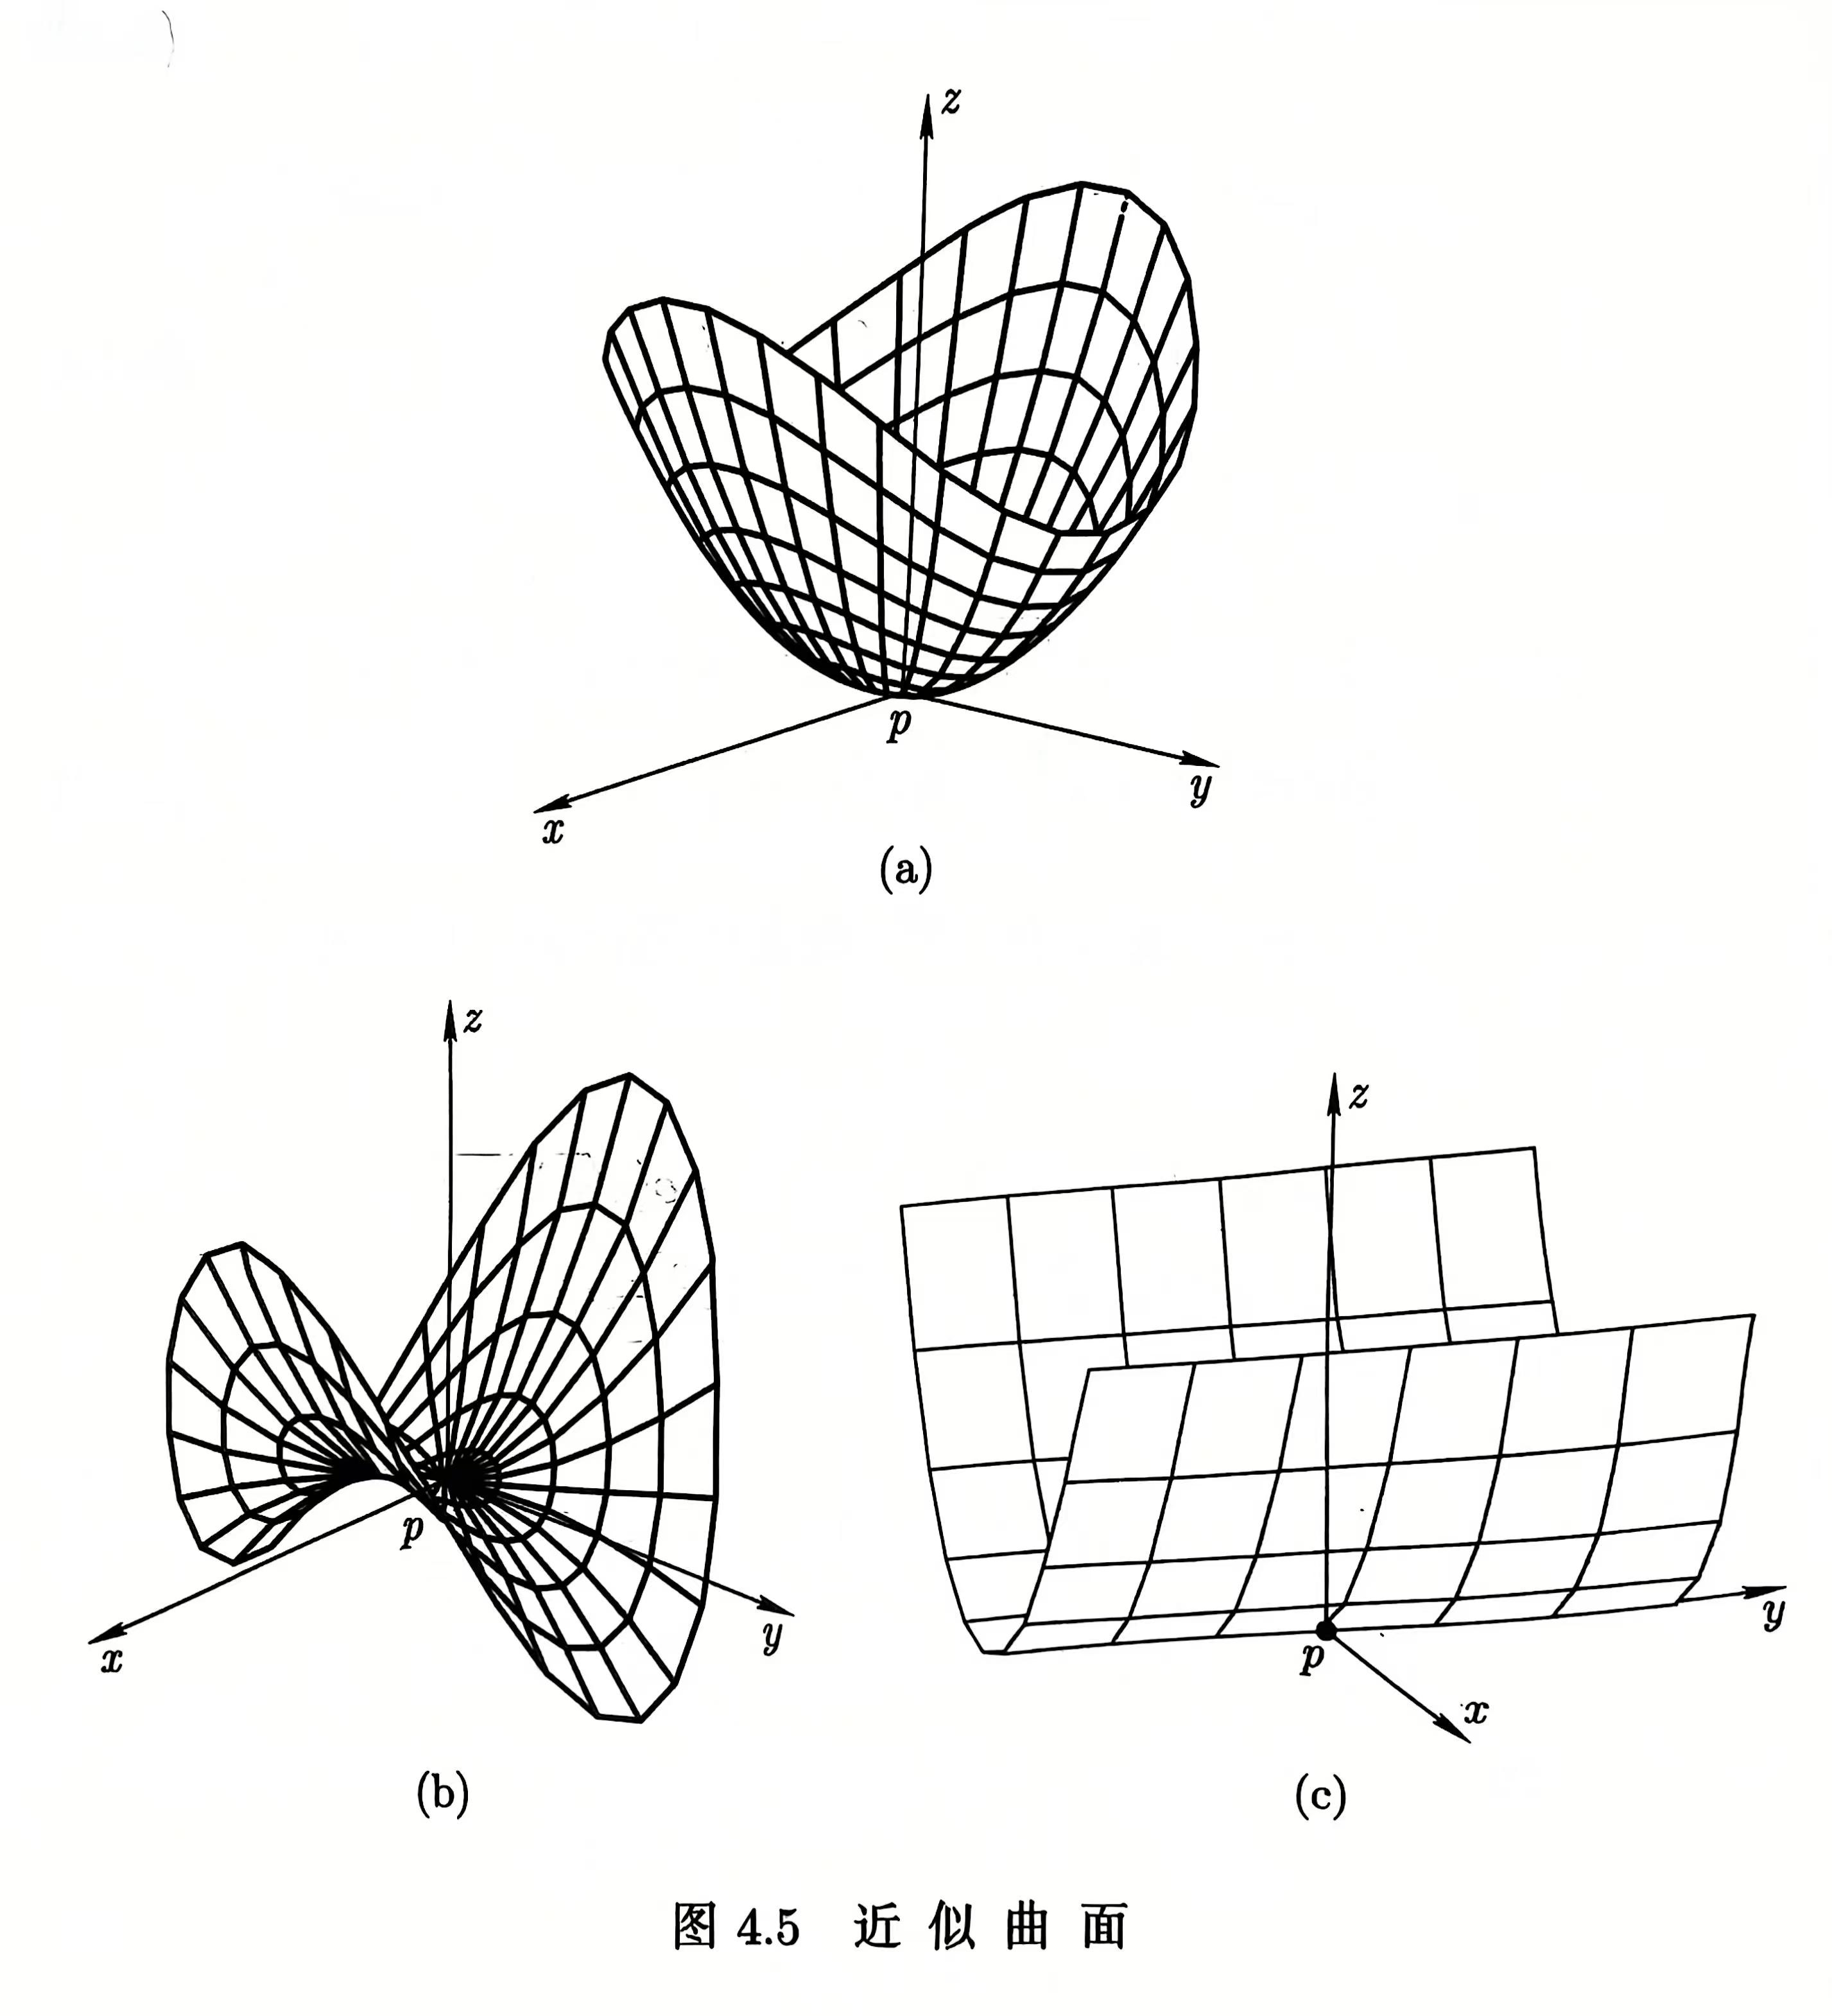
\includegraphics[width=0.4\textwidth]{dupin.jpg}
    \caption{三种近似曲面}
\end{figure}

本章最后还介绍了\textbf{条件极值}的概念与\textbf{拉格朗日乘数法}.
这些内容本身不难，但是可以出成压轴的计算题，因此需要认真练习掌握.
需要提醒的是，拉格朗日乘数法求解的结果只是得到了稳定点，而稳定点未必一定是极值点，需要进行检验.\par

\subsubsection{补充说明}\par
（1）只有当$f_{xy}$和$f_{yx}$都连续时，它们才相等.
在实际应用中，$f_{xy} = f_{yx}$是常态，因此可以不假思索地认为它成立.
但是作为数学课，还是应该有“二阶偏导不一定连续”的意识.
 \par
（2）多元函数微分学的建立仍然没有离开数学分析的体系.
多元函数的极限、连续、偏导数等概念都有其$\epsilon - \delta$语言的定义，
相关引申结论也可以用$\epsilon - \delta$语言来证明.
虽然在高数学习中已经不强调了，但是在学有余力的情况下最好还是掌握定理的证明.\par
（3）第10节“曲面论引论”的内容不在考试范围内，但是在高数下会有用.
有空可以看一看.\par

\subsection{解题方法}

\subsubsection{二元函数的极限计算}

\textbf{1.~~证明极限不存在(尝试三条特殊路径)} \vspace{0.25em}

要证明一个函数极限不存在，只需要举出两条不同的路径，
使得点$P$沿这两条路径趋向$P_0$时取得的极限值不同.
一般来说，当我们拿到一个陌生的二元函数时，可以先取几条路径试试看.
如果几番尝试都找不到两条极限值不同的路径，
那么可以开始尝试证明二元函数的极限存在.

根据往年题的经验，若题目所给的函数真的不存在极限，那么三步之内必现端倪——设待求极限的点$P_0$为$(0,0)$，则只需尝试以下三条路径：\par
(1)~$y = 0 ~~(x \to 0)$;\par
(2)~$x = 0 ~~(y \to 0)$;\par
(3)~$y = x~~(x \to 0)$;\par
保险起见，可以再检查一切的直线路径，即：\par
(4)~$y = kx~~(x \to 0)$.

\begin{example}[2020]
\label{ex:ch06-01}
二元函数极限$\lim\limits_{\scriptscriptstyle{(x,y)\to (0,0)} }\frac{x^5y^3}{x^8+y^8}$是否存在？
若存在，求出极限值；若不存在，写出理由.
\end{example}

\begin{solution}
不存在. 取路径$y = 0 ~~(x \to 0)$：
$$
\limx0 \frac{x^5 \cdot 0^3}{x^8+0^8} = 0
$$\par
取路径$y = x~~(x \to 0)$：
$$
\limx0 \frac{x^5 \cdot x^3}{x^8 + x^8} = \frac{1}{2}
$$\par
沿这两条路径的极限值不同，因此二元函数的极限不存在.
\end{solution}

\begin{example}[2022 A卷]
\label{ex:ch06-02}
二元函数极限
$\lim\limits_{\scriptscriptstyle{(x,y)\to (0,0)} }\frac{x \sin y}{(\sin x)^2 + (\sin y)^2}$
是否存在？
若存在，求出极限值；若不存在，写出理由.
\end{example}

\begin{solution}
不存在. 取路径$y = 0 ~~(x \to 0)$：
$$
\limx0 \frac{x \cdot \sin 0}{(\sin x)^2+ (\sin 0)^2} = 0
$$\par
取路径$y = x~~(x \to 0)$：
$$
\limx0 \frac{x \cdot \sin x}{(\sin x)^2 + (\sin x)^2} = \frac{1}{2}
$$

沿这两条路径的极限值不同，因此二元函数的极限不存在.
\end{solution}

\begin{example}[2022 B卷]
\label{ex:ch06-03}
二元函数极限
$\lim\limits_{\scriptscriptstyle{(x,y)\to (0,0)} }\frac{xy}{x^2 + (e^y - 1)^2}$
是否存在？
若存在，求出极限值；若不存在，写出理由.
\end{example}

\begin{solution}
不存在. 取路径$y = 0 ~~(x \to 0)$：
$$
\limx0 \frac{x \cdot 0}{x^2+ (e^0 - 1)^2} = 0
$$\par
取路径$y = x~~(x \to 0)$：
$$
\limx0 \frac{x \cdot x}{x^2 + (e^x -1)^2} = \limx0 \frac{1}{1 + \left( \displaystyle\frac{e^x - 1}{x} \right)^2} = \frac{1}{2}
$$\par
沿这两条路径的极限值不同，因此二元函数的极限不存在.
\end{solution}

\textbf{2.证明极限存在(夹逼定理、换元法)} \vspace{0.25em}

若尝试了所有直线路径，发现极限值并无不同，则可以猜测二元函数极限存在. 具体思路一般只有两种：\par
(1)~用夹逼定理：关键是把二元函数拆成两项的乘积，其中一半（在邻域内）是有界的，可以放缩至常数；另一半的极限为0.
这种情况下可以轻易证明两部分相乘的极限为0.\par
(2)~换元法：利用复合函数极限的性质，将二元函数的极限化为一元函数的极限.

\begin{example}[2020]
\label{ex:ch06-04}
二元函数极限
$\lim\limits_{\scriptscriptstyle{(x,y)\to (0,0)} } (x + \sin y) ~\cos \frac{1}{|x|+|y|}$
是否存在？
若存在，求出极限值；若不存在，写出理由.
\end{example}

\begin{solution}
用夹逼定理证明该极限存在且等于$0$. 由$-1 \le \cos \frac{1}{|x|+|y|} \le 1$，得：
$$
-|x+\sin y| ~\le~ (x+\sin y) \cos \frac{1}{|x|+|y|} ~\le~ \left| x+\sin y \right|
$$\par
对不等式链的最左侧和最右侧取极限. 由极限的加法和复合函数的极限可知：
$$
\lim\limits_{\scriptscriptstyle{(x,y)\to (0,0)} } -|x+\sin y| = 0~~,
\lim\limits_{\scriptscriptstyle{(x,y)\to (0,0)} } |x+\sin y| = 0
$$

因此根据夹逼定理，$\lim\limits_{\scriptscriptstyle{(x,y)\to (0,0)} } (x + \sin y) ~\cos \frac{1}{|x|+|y|} = 0$.
\end{solution}

（注：由于$x + \sin y$的正负不定，在放缩时应该加上绝对值.
2020$\sim$21高数B期末考试答案文档中没有如此做，可能并不严谨.）

\begin{example}[2022 A卷]
\label{ex:ch06-05}
二元函数极限
$\lim\limits_{\scriptscriptstyle{(x,y)\to (0,0)} } \left(x + \ln(1+y)\right) \cos \frac{1}{x^2+y^2}$
是否存在？
若存在，求出极限值；若不存在，写出理由.
\end{example}

\begin{solution}
用夹逼定理证明该极限存在且等于$0$.由$-1 \le \cos \frac{1}{x^2 + y^2} \le 1$，得：
$$
- \left| x + \ln(1+y) \right|
~\le~
\left(x + \ln(1+y)\right) \cos \frac{1}{x^2+y^2}
~\le~
\left| x + \ln(1+y) \right|
$$\par
对不等式链的最左侧和最右侧取极限. 由极限的加法和复合函数的极限可知：
$$
\lim\limits_{\scriptscriptstyle{(x,y)\to (0,0)} } -\left| x + \ln(1+y) \right| = 0~~,
\lim\limits_{\scriptscriptstyle{(x,y)\to (0,0)} } \left| x + \ln(1+y) \right| = 0
$$\par
因此根据夹逼定理，$\lim\limits_{\scriptscriptstyle{(x,y)\to (0,0)} } \left(x + \ln(1+y)\right) \cos \frac{1}{x^2+y^2} = 0$.
\end{solution}

\begin{example}[2022 B卷]
\label{ex:ch06-06}
二元函数极限
$\lim\limits_{\scriptscriptstyle{(x,y)\to (0,0)} } \left(e^y - 1\right) \frac{xy}{x^2 + y^2}$.
是否存在？
若存在，求出极限值；若不存在，写出理由.
\end{example}

\begin{solution}
用夹逼定理证明该极限存在且等于$0$. 由基本不等式$- \frac{x^2 + y^2}{2} \le xy \le \frac{x^2 + y^2}{2}$，有：
$$
-\frac{1}{2} \le \frac{xy}{x^2 + y^2}  \le  \frac{1}{2}
$$\par
从而：
$$
-\frac{1}{2}|e^y - 1|
~\le~
\left(e^y - 1\right)\frac{xy}{x^2 + y^2}
~\le~
\frac{1}{2}|e^y - 1|
$$\par
对不等式链的最左侧和最右侧取极限：
$$
\lim\limits_{\scriptscriptstyle{(x,y)\to (0,0)} } -\frac{1}{2}|e^y - 1|  = 0~~,
\lim\limits_{\scriptscriptstyle{(x,y)\to (0,0)} } \frac{1}{2}|e^y - 1| = 0
$$

因此根据夹逼定理，$\lim\limits_{\scriptscriptstyle{(x,y)\to (0,0)} } \left(e^y - 1\right) \frac{xy}{x^2 + y^2} = 0$.
\end{solution}

\begin{example}[2022 A卷]
\label{ex:ch06-07}
二元函数极限
$\lim\limits_{\scriptscriptstyle{(x,y)\to (0,0)} } \frac{24\cos \sqrt{x^2 + y^2} - 24 + 12(x^2 + y^2)}{( \tan \sqrt{x^2 + y^2})^4}$.
是否存在？
若存在，求出极限值；若不存在，写出理由.
\end{example}

\begin{solution}
令$r(x,y) = \sqrt{x^2 + y^2}$，则当$(x,y) \to (0,0)$时，$r \to 0$.
由复合函数的极限可知：
\begin{equation}
    \begin{aligned}
        \lim\limits_{\scriptscriptstyle{(x,y)\to (0,0)} } \frac{24\cos \sqrt{x^2 + y^2} - 24 + 12(x^2 + y^2)}{( \tan \sqrt{x^2 + y^2})^4}
        &= \lim\limits_{r \to 0} \frac{24\cos r -24 + 12r^2}{\tan^4 r} \\
        &= \lim\limits_{r \to 0} \frac{24(1 - \displaystyle\frac{r^2}{2} + \displaystyle\frac{r^4}{4!} + o(r^4)) -24 + 12r^2}{r^4} \\
        &= 1
        \nonumber
    \end{aligned}
\end{equation}
\end{solution}

\subsubsection{连续性与可微性的判断}\par
判断一个多元函数在某点处是否连续，只需要判断极限是否存在，函数值是否等于极限值.\par
判断一个多元函数在某点$P$处是否可微，也需要直接使用定义——\textbf{全增量}可以表示为\textbf{线性主要部分}加上一个高阶无穷小量$o(\rho)$.
其中$\rho$是指$P$到原点$O$的距离.
具体做法时，先计算函数对各个变量的偏导数，从而得到线性主要部分.
将$P$点的函数值减去线性主要部分，然后判断剩余部分是否为$\rho$的高阶无穷小量.\par
往年题和习题书中的套路一般是这样的：可以证明到函数连续，并且偏导数存在，最后一问要去证明不可微.
假设连偏导数都不存在，那就可以直接说不可微了.

\begin{example}[2021]
\label{ex:ch06-08}
定义三元函数$f:~\mathbb{R}^3 \to \mathbb{R}$为：
\[ \setstretch{1.5}
f(x,y,z) =
\begin{cases}
    \frac{xyz}{x^2 + y^2 + z^2} &\quad \text{当}(x,y,z) \ne (0,0,0) \\
    0  &\quad \text{当}(x,y,z) = (0,0,0)
\end{cases}
\] \setstretch{1.75}
\par
(1)~计算出$f$在点$(0,0,0)$处三个偏导数$f_{x}(0,0,0)$，$f_{y}(0,0,0)$，$f_z(0,0,0)$.\par
(2)~三元函数$f$在点$(0,0,0)$处可微吗？证明你的结论.
\end{example}

\begin{solution}
(1)~~偏导数的计算方法实质上是一元函数的导数，因此根据定义：
$$
f_{x}(0,0,0) = \limx0 \frac{f(x,0,0) - f(0,0,0)}{x}
= \limx0 \frac{\dfrac{x \cdot 0 \cdot 0}{x^2 + 0^2 + 0^2} - 0}{x} = 0
$$

同理，可以计算得到$f_{y}(0,0,0) = f_{z}(0,0,0) = 0$.

(2)~~三元函数$f$在点$(0,0,0)$不可微. 证明如下：

用反证法. 如果可微，根据定义，$f(x,y,z)$可以写成：
\begin{eq}
    f(x,y,z) &= f(0,0,0) + f_{x}(0,0,0)\cdot x + f_{y}(0,0,0)\cdot y + f_{z}(0,0,0)\cdot z + o(\rho)
\end{eq}

其中$\rho = \sqrt{x^2 + y^2 + z^2}$.
代入各偏导数、$f(x,y,z)$（$x,y,z \ne 0$）和$f(0,0,0)$的值，整理，得到：
$$
o(\rho) = \frac{xyz}{x^2 + y^2 + z^2}
$$

根据高阶无穷小量的定义，这等价于：
$$
\lim\limits_{(x,y,z) \to (0,0,0)} \frac{xyz}{(x^2 + y^2 + z^2)\rho} =
\lim\limits_{(x,y,z) \to (0,0,0)} \frac{xyz}{(x^2 + y^2 + z^2)^\frac{3}{2}} = 0
$$

但这个极限事实上是不存在的.
因为取特殊路径$y=z=0$时，
$\limx0 \frac{x \cdot 0 \cdot 0}{x^2 + 0^2 + 0^2} = 0$；而取特殊路径$x=y=z$时：
$\limx0 \frac{x \cdot x \cdot x}{(x^2 + x^2 + x^2)^\frac{3}{2}} = \frac{1}{3\sqrt{3}} \ne 0$.
因此$f$在点$(0,0,0)$处不可微.
\end{solution}

\begin{example}
\label{ex:ch06-09}
设函数：
\[ f(x,y) =
\begin{cases}
    \frac{x^3 + y^3}{x^2 + y^2} &\quad \text{当}(x,y) \ne (0,0) \\
    0  &\quad \text{当}(x,y) = (0,0)
\end{cases}
\]

(1)~函数$f(x,y)$在点$(0,0)$处是否连续？

(2)~函数$f(x,y)$在点$(0,0)$处的两个一阶偏导数是否存在？若存在，求出这两个偏导数.

(3)~函数$f(x,y)$在点$(0,0)$处是否可微？若可微，求出函数的微分.
\end{example}

\begin{solution}
(1)~~如果不连续，最后一小问就没得做了，所以必然连续.
证明如下：

只需证明$f(x,y)$在点$(0,0)$处的极限为$0$.
为了用夹逼定理，对$|f(x,y)|$进行放缩：
$$
0 \le \left| \frac{x^3 + y^3}{x^2 + y^2} \right|
\le \frac{|x^3|}{x^2 + y^2} + \frac{|y^3|}{x^2 + y^2}
\le |x| + |y|
$$

不等式链的最左侧和最右侧在$(x,y) \to (0,0)$时均趋向于$0$.
根据夹逼定理，被夹的函数$|f|$极限也为$0$.
因此函数$f(x,y)$在点$(0,0)$处的极限为$0$，且等于$f(0,0)$，
从而函数$f(x,y)$在点$(0,0)$处连续.

(2)~~由偏导数定义：
$$
f_x(0,0) = \limx0 \frac{f(x,0) - f(0,0)}{x} = 1
$$\par
同理，计算得到$f_y(0,0) = 1$.

(3)~~不可微. 证明如下：
用反证法. 如果可微，根据定义，$f(x,y)$可以写成：
\begin{equation}
    \begin{aligned}
        f(x,y) &= f(0,0) + f_{x}(0,0)\cdot x + f_{y}(0,0)\cdot y + o(\rho)
        \nonumber
    \end{aligned}
\end{equation}

其中$\rho = \sqrt{x^2 + y^2}$. 代入各偏导数、$f(x,y)$（$x,y \ne 0$）和$f(0,0)$的值，整理，得到：
$$
o(\rho) = \frac{x^3 + y^3}{x^2 + y^2} - x - y = \frac{-xy(x+y)}{x^2 + y^2}
$$

根据高阶无穷小量的定义，这等价于：
$$
\lim\limits_{(x,y) \to (0,0)} \frac{-xy(x+y)}{(x^2 + y^2)\rho} =
\lim\limits_{(x,y) \to (0,0)} \frac{-xy(x+y)}{(x^2 + y^2)^\frac{3}{2}} = 0
$$

但这个极限事实上是不存在的. 因为取特殊路径$y=0$时：
$\limx0 \frac{0}{(x^2 + 0^2)^\frac{3}{2}} = 0$；
而取特殊路径$y=x$时：
$\limx0 \frac{-x \cdot x \cdot (x+x)}{(x^2 + x^2)^{\frac{3}{2}}} = \frac{1}{\sqrt{2}} \ne 0$.
因此$f$在点$(0,0)$处不可微.
\end{solution}

\subsubsection{多元函数求导}
考试中一般会有一种无聊的题型，就是直接给一个复合函数，要求通过求各种导数来计算某个式子或者验证某个等式.\par
这种题目没有任何技巧，就靠硬算.
我们先借一道相对较难的题目带大家复习复合函数求导的方法.

\begin{example}
\label{ex:ch06-10}
已知函数$z = f(xy,e^{x+y})$，且$f(x,y)$具有连续二阶偏导数. 计算$\frac{\partial^2 z}{\partial x \partial y}$.
\end{example}

\begin{solution}
这是一个复合函数. 设$z = f(u,v)$，其中$u(x,y) = xy$，$v(x,y) = e^{x+y}$.
先对$y$求偏导：

\begin{equation}
    \begin{aligned}
        \frac{\partial z}{\partial y} &= \frac{\partial z}{\partial u} \frac{\partial u}{\partial y} +
                                        \frac{\partial z}{\partial v} \frac{\partial v}{\partial y} \\
        &= f_u(xy,e^{x+y}) \cdot x + f_v(xy,e^{x+y}) \cdot e^{x+y}
        \nonumber
    \end{aligned}
\end{equation}

\setstretch{2}
（在上面的计算步骤中，$\frac{\partial z}{\partial u}$和$f_u(xy,e^{x+y})$是同一个东西，只是换了个写法.
$\frac{\partial z}{\partial v}$也是一样.
之所以这样写，是为了强调$\frac{\partial z}{\partial u}$也是与$x$和$y$有关的二元函数.
在后续的求导过程中，不能忘记对偏导数再求偏导数.）

\setstretch{1.75}

然后再对$x$求偏导.
这时要注意，对$\frac{\partial z}{\partial u}$求偏导还是会出来两项.
还要注意函数乘积的求导，
\begin{equation}
    \begin{aligned}
        \frac{\partial^2}{\partial x \partial y}
        &= f_{uu}(xy,e^{x+y})\cdot xy + f_{uv}(xy,e^{x+y}) \cdot xe^{x+y} + f_u(xy,e^{x+y}) \\
        &~~~~+ f_{vu}(xy,e^{x+y}) \cdot ye^{x+y} + f_{vv}(xy,e^{x+y}) \cdot e^{2x+2y} + f_v(xy,e^{x+y}) \cdot e^{x+y} \\
        &= f_{uu}(xy,e^{x+y})\cdot xy + f_{uv}(xy,e^{x+y}) \cdot (x+y)e^{x+y} + f_{vv}(xy,e^{x+y}) \cdot e^{2x+2y} \\
        &~~~~+ f_u(xy,e^{x+y}) + f_v(xy,e^{x+y}) \cdot e^{x+y}
        \nonumber
    \end{aligned}
\end{equation}

由于$f$是题目给定的二元函数，其偏导数$f_u$和$f_v$是已知的.
所以本题到此为止已经做完.
有同学可能担心，$u$和$v$是我们解题时引入的变量，在答案中出现是不是不太好？
为了避免这个问题，可以用$f_1$来表示“$f$对第一分量求偏导”，用$f_2$来表示“$f$对第二分量求偏导”.
于是答案可以写成：
$$
\frac{\partial^2}{\partial x \partial y}
= xyf_{11} + (x+y)e^{x+y} f_{12} + e^{2x+2y} f_{22} + f_1 + e^{x+y} f_2
$$
\end{solution}

例\ref{ex:ch06-10}涉及到对抽象复合函数$f$求二阶偏导，展开的项数较多，对链式法则的熟练程度提出了一定的要求.
如果会做这道题，那么期末考试的题目就没有什么可怕的.
但是，一些题目的计算量可能比较大，计算时要小心.

这里一并把所有求导相关的题目都做一个说明.
存在一些所谓的“应用题”，要求计算梯度或者方向导数.
有的题目会问“函数值下降最快的方向”，其实就是指负梯度方向.
另外，后续要用到隐函数存在定理的一些题目，可能会要求计算切线方程.
以上种种变化，都逃不开求偏导数.
无论是方向导数、梯度、还是切线方程，只要知道了偏导数，根据各自的定义就可以轻易算出来.

\begin{example}[2021]
\label{ex:ch06-11}
设$f:~\mathbb{R} \to \mathbb{R}$和$g:~\mathbb{R} \to \mathbb{R}$
都有连续的二阶导函数. 任给$x \in \mathbb{R}$，$y \in \mathbb{R}$，
当$x \ne 0$时，定义：
$$
h(x,y) = x~f\left(\frac{y}{x}\right) ~+~ g\left(\frac{y}{x}\right)
$$

计算出：
$$
x^2 ~h_{xx}(x,y) + 2xy~ h_{yx}(x,y) + y^2 ~h_{yy}(x,y)
$$
\end{example}

\begin{solution}
先计算两个一阶偏导数：
$$
h_{x}(x,y) = f\left(\frac{y}{x}\right) -  \frac{y}{x} f'\left(\frac{y}{x}\right) - \frac{y}{x^2}g'\left(\frac{y}{x}\right)
$$
$$
h_{y}(x,y) = f'\left(\frac{y}{x}\right) + \frac{1}{x}g'\left(\frac{y}{x}\right)
$$\par
再计算三个二阶偏导数：
\begin{equation}
    \begin{aligned}
    h_{xx}(x,y) &~=~ \frac{-y}{x^2}f'\left(\frac{y}{x}\right)
    ~+~ \frac{y}{x^2}f'\left(\frac{y}{x}\right)
    ~+~ \frac{y^2}{x^3}f''\left(\frac{y}{x}\right)
    ~+~ \frac{2y}{x^3}g'\left(\frac{y}{x}\right)
    ~+~ \frac{y^2}{x^4}g''\left(\frac{y}{x}\right) \\
    &~=~ \frac{y^2}{x^3}f''\left(\frac{y}{x}\right)
    ~+~ \frac{2y}{x^3}g'\left(\frac{y}{x}\right)
    ~+~ \frac{y^2}{x^4}g''\left(\frac{y}{x}\right) \\
    h_{yx}(x,y) &~=~ \frac{-y}{x^2} f''\left(\frac{y}{x}\right)
    ~-~\frac{1}{x^2}g'\left(\frac{y}{x}\right)
    ~-~\frac{y}{x^3}g''\left(\frac{y}{x}\right) \\
    h_{yy}(x,y) &~=~ \frac{1}{x}f''\left(\frac{y}{x}\right)
    ~+~ \frac{1}{x^2}g''\left(\frac{y}{x}\right)
    \nonumber
    \end{aligned}
\end{equation} \par
合起来代入表达式：
\begin{equation}
    \begin{aligned}
        x^2 h_{xx}(x,y) + 2xy h_{yx}(x,y) + y^2 h_{yy}(x,y)
        &= x^2 \left( \frac{y^2}{x^3}f''\left(\frac{y}{x}\right)
        ~+~ \frac{2y}{x^3}g'\left(\frac{y}{x}\right)
        ~+~ \frac{y^2}{x^4}g''\left(\frac{y}{x}\right) \right) \\
        &~~~~~~+~ 2xy \left( \frac{-y}{x^2} f''\left(\frac{y}{x}\right)
        ~-~\frac{1}{x^2}g'\left(\frac{y}{x}\right)
        ~-~\frac{y}{x^3}g''\left(\frac{y}{x}\right) \right) \\
        &~~~~~~+~y^2 \left( \frac{1}{x}f''\left(\frac{y}{x}\right)
        ~+~ \frac{1}{x^2}g''\left(\frac{y}{x}\right)\right) \\
        &~=~  \left( \frac{y^2}{x}f''\left(\frac{y}{x}\right)
        ~+~ \frac{2y}{x}g'\left(\frac{y}{x}\right)
        ~+~ \frac{y^2}{x^2}g''\left(\frac{y}{x}\right) \right) \\
        &~~~~~~+~  \left( -\frac{2y^2}{x} f''\left(\frac{y}{x}\right)
        ~-~\frac{2y}{x}g'\left(\frac{y}{x}\right)
        ~-~\frac{2y^2}{x^2}g''\left(\frac{y}{x}\right) \right) \\
        &~~~~~~+~  \left( \frac{y^2}{x}f''\left(\frac{y}{x}\right)
        ~+~ \frac{y^2}{x^2}g''\left(\frac{y}{x}\right) \right) \\
        &~=~0
        \nonumber
    \end{aligned}
\end{equation}
\end{solution}

\begin{example}[2020]
\label{ex:ch06-12}
设在空间$\mathbb{R}^3$中$Oxy$平面之外的点$(x,y,z)$电势
$V = \left( \frac{2y}{z} \right)^x$.
求出在点$(1,\frac{1}{2},1)$处，电势$V$下降最快的方向上的单位向量.
\end{example}

\begin{solution}
$$
V_{x}(1,\frac{1}{2},1) = \left( \frac{2y}{z}\right)^{x} \cdot \ln \left(\frac{2y}{z} \right) \bigg|_{(1,\frac{1}{2},1)} = 0
$$
$$
V_{y}(1,\frac{1}{2},1) = x \cdot \left( \frac{2y}{z}\right)^{x-1} \cdot \frac{2}{z} \bigg|_{(1,\frac{1}{2},1)} = 2
$$
$$
V_{z}(1,\frac{1}{2},1) = x \cdot \left( \frac{2y}{z}\right)^{x-1} \cdot \left( -\frac{2y}{x^2} \right) \bigg|_{(1,\frac{1}{2},1)} = -1
$$

电势$V$下降最快的方向即为负的梯度方向. 先计算梯度：
$$
\bm{-E} =
\mathbf{grad}~V \bigg|_{(1,\frac{1}{2},1)}
= (V_x,V_y,V_z) \bigg|_{(1,\frac{1}{2},1)}
= (0,2,-1)
$$

因此电势下降最快的方向的单位向量是：
$$
\bm{e}_{E} = \frac{\bm{E}}{|\bm{E}|} = \left( 0,-\frac{2}{\sqrt{5}},\frac{1}{\sqrt{5}} \right)
$$

（注：电势$V$的负梯度就是电场强度$\bm{E}$.
原答案文档中可能想通过$E$这个字母偷偷揭示这一点，但是弄错了正负号. 答案没有错.）
\end{solution}

\begin{example}[2022 B卷]
\label{ex:ch06-13}
设整数$n \ge 3$，定义$n$元函数：
$$
u(x_1,x_2, \cdots ,x_n) = \left( \sum_{k=1}^{n} x_{k}^{2} \right)^{1-n/2}
$$

其中$\sum_{k=1}^{n} x_{k}^{2} \ne 0$.
计算出$\sum_{k=1}^{n} u_{x_k x_k}$.
\end{example}

\begin{solution}
先计算一阶导数：
\begin{equation}
    \begin{aligned}
        u_{x_k} &=
        \frac{2-n}{2} \left( x_1^2 + \cdots + x_n^2 \right)^{-n/2} \cdot 2x_k \\
        &=  (2-n)\left( x_1^2 + \cdots + x_n^2 \right)^{-n/2} \cdot x_k
        \nonumber
    \end{aligned}
\end{equation}\par
再计算二阶导数：
\begin{equation}
    \begin{aligned}
        u_{x_k x_k} &=
        (2-n) \left[ \left( x_1^2 + \cdots + x_n^2 \right)^{-n/2} + \left(-\frac{n}{2}\right) \left( x_1^2 + \cdots + x_n^2 \right)^{-n/2-1}\cdot 2x_k^2 \right] \\
        &= (2-n) \left( x_1^2 + \cdots + x_n^2 \right)^{-n/2-1} \left[ \left( x_1^2 + \cdots + x_n^2 \right) -n x_k^2 \right]
        \nonumber
    \end{aligned}
\end{equation}

于是：
\begin{eq1}
    \sum_{k=1}^{n} u_{x_k x_k} =
(2-n) \left( x_1^2 + \cdots + x_n^2 \right)^{-\frac{n}{2}-1} \left[ n \left( x_1^2 + \cdots + x_n^2 \right) -n \left( x_1^2 + \cdots + x_n^2 \right) \right]
=0
\end{eq1}
\end{solution}

\begin{example}[2022 B卷]
\label{ex:ch06-14}
设二元函数$h(x,t) = f(x+at)+g(x-at)$，
其中$f:~\mathbb{R} \to \mathbb{R}$和$g:~\mathbb{R} \to \mathbb{R}$都有二阶导函数，$a$是常数.
计算出$h_{tt} - a^2 h_{xx}$.
\end{example}

\begin{solution}
先计算各个一阶导数，再计算各个二阶导数：
\begin{eq1}
    h_{t} &= af'(x+at) -a g'(x-at) \\
    h_x &= f'(x+at) + g'(x -at) \\
    h_{tt} &= a^2 f''(x+at) + a^2 g''(x-at) \\
    h_{xx} &= f''(x+at) + g''(x-at)
\end{eq1}

代入表达式，得到$h_{tt} - a^2 h_{xx} = 0$.
\end{solution}

（注：此题验证了$h(x,t)$是波动方程行波解的一般形式.）

\begin{example}[2023]
\label{ex:ch06-15}
(1)~举例说明：当$z$是$(x,y)$的函数，也是$(t,u)$的函数时，$x$恒等于$t$推不出$\frac{\partial z}{\partial x}$恒等于$\frac{\partial z}{\partial t}$.

(2)~给定方程：$x^2~ \frac{\partial z}{\partial x} ~+~ y^2~ \frac{\partial z}{\partial y} = z^2 $.
作变量代换$x = t$，$y = \frac{t}{1+tu}$，$z = \frac{t}{1+tW}$.
证明：$\frac{\partial W}{\partial t} = 0$.
\end{example}

\begin{analysis}
将同一个变量$z$用两组不同的自变量来表示，
相当于用两个不同的坐标系来描述同一张曲面.
既然坐标系都不同了，同一张曲面的方程很有可能也是不同的.
那么偏导数不同也是很正常的.
\end{analysis}

\begin{solution}
(1)~~例如$z=f(x,y)=x+y$，$z=g(t,u) = 2t+u$. 两组自变量之间满足变换关系$t=x$，$u=y-x$.
则有：
$$
\frac{\partial z}{\partial x} = \frac{\partial f(x,y)}{\partial x} = 1
$$
$$
\frac{\partial z}{\partial t} = \frac{\partial g(t,u)}{\partial t} = 2
$$\par
可见$\frac{\partial z}{\partial x}$并不恒等于$\frac{\partial z}{\partial t}$.\par

(2)~~要计算$\frac{\partial W}{\partial t}$，最好是写出$W$的显函数表达式. 在本题中这是很容易做到的.
对$z$的变量代换式进行整理，得到：
$$
W = \frac{1}{z} - \frac{1}{t}
$$
现在要利用这个表达式来计算$\frac{\partial W}{\partial t}$.
根据上一小问的提示，$z$原本是关于$x$和$y$的函数，做变量代换之后又变成了关于$t$和$u$的函数.
为了避免混淆这两个函数关系，可以设$z = f(x,y) = g(t,u)$.
这样$\frac{\partial z}{\partial x}$就是指$\frac{\partial f}{\partial x}$，
$\frac{\partial z}{\partial t}$就是指$\frac{\partial g}{\partial t}$.
明确了这一点，我们计算$W$对$t$的偏导数，要把它当成复合函数处理.
这样还便于利用本小问给定的方程.
\begin{equation}
    \begin{aligned}
        \frac{\partial W}{\partial t} &= -\frac{1}{z^2} \frac{\partial z}{\partial t} + \frac{1}{t^2} \\
        &= -\frac{1}{z^2} \left( \frac{\partial z}{\partial x} \frac{\partial x}{\partial t} + \frac{\partial z}{\partial y} \frac{\partial y}{\partial t} \right)
        + \frac{1}{t^2}
        \nonumber
    \end{aligned}
\end{equation}\par
由变量代换式$x = t$和$y = \frac{t}{1 + tu}$可以分别直接计算得到$\frac{\partial x}{\partial t}=1$和
$\frac{\partial y}{\partial t} = \frac{1}{(1 + tu)^2} = \frac{y^2}{t^2} = \frac{y^2}{x^2}$.
代入$\frac{\partial W}{\partial t}$的表达式，有：
$$
\frac{\partial W}{\partial t}  =
-\frac{1}{z^2} \left( \frac{\partial z}{\partial x} + \frac{\partial z}{\partial y}\cdot \frac{y^2}{x^2} \right) + \frac{1}{t^2}
$$

将括号里的式子与本小问题干所给的方程进行比较，发现只差了一个倍数$x^2$.
因此利用方程可以彻底地化简：
$$
\frac{\partial W}{\partial t}  ~= ~
-\frac{1}{z^2} \cdot \frac{z^2}{x^2} + \frac{1}{t^2} ~=~ -\frac{1}{z^2} \cdot \frac{z^2}{t^2} + \frac{1}{t^2}~=~ 0
$$
\end{solution}

\subsubsection{隐函数}

\begin{example}[2022 A卷]
\label{ex:ch06-16}
证明：任意给定实数$k$，存在点$0$的开邻域$U$，存在点$0$的开邻域$W$，
存在唯一的函数$y=f(x)$，$x \in U$，$y \in W$满足方程
$e^{kx} + e^{ky} - 2e^{x+y} = 0$.
\end{example}

\begin{proof}
先尝试验证题设满足隐函数存在定理的条件.
令等号左边为一个二元函数$F(x,y) = e^{kx} + e^{ky} - 2e^{x+y}$.
则$F(x,y)$在$\mathbb{R}^2$上处处有定义，
且$F(0,0) = 0$.\par
计算$F(x,y)$的两个偏导数：
\begin{equation}
    \begin{aligned}
        F_{x}(x,y) &= k e^{kx} - 2e^{x+y} \\
        F_{y}(x,y) &= k e^{ky} -2e^{x+y}
        \nonumber
    \end{aligned}
\end{equation}\par
二者都是$\mathbb{R}^2$中的连续函数，且$F_{y}(0,0) = k - 2$.
当$k \ne 2$时，$F_{y}(0,0) \ne 0$.
以上验证了隐函数存在定理的全部条件.
因此在$(0,0)$的某个邻域内存在唯一的函数$y=f(x)$满足方程.\par
当$k = 2$时，$F(x,y) = (e^x - e^y)^2$. $F(x,y)= 0$当且仅当$x=y$，
即确定了唯一的隐函数$y = f(x) = x$.
\end{proof}

\begin{example}[2022 B卷]
\label{ex:ch06-17}
证明：任意给定实数$k$，存在点$1$的开邻域$U$，存在点$1$的开邻域$W$，
存在唯一的函数$y=f(x)$，$x \in U$，$y \in W$满足方程
$x^k - 3x^2 y + 3x y^2 - y^k = 0$.
\end{example}

\begin{proof}
只需验证题设满足隐函数存在定理的条件.
令等号左边为一个二元函数$F(x,y) = x^k - 3x^2 y + 3x y^2 - y^k$.
则$F(x,y)$在$\mathbb{R}^2$上处处有定义，
且$F(1,1) = 0$.\par
计算$F(x,y)$的两个偏导数：
\begin{equation}
    \begin{aligned}
        F_{x}(x,y) &= k x^{k-1} -6xy + 3y^2 \\
        F_{y}(x,y) &= -3x^2 + 6xy -k y^{k-1}
        \nonumber
    \end{aligned}
\end{equation}\par
二者都是$\mathbb{R}^2$中的连续函数，且$F_{y}(1,1) = 3-k$.
当$k \ne 3$时，$F_{y}(1,1) \ne 0$.
以上验证了隐函数存在定理的全部条件.
因此在$(1,1)$的某个邻域内存在唯一的函数$y=f(x)$满足方程.\par
当$k = 3$时，$F(x,y) = (x - y)^3$. $F(x,y)= 0$当且仅当$y=x$.
这也在$(1,1)$的邻域内确定了惟一符合要求的函数$f$.
\end{proof}

\begin{example}[2022 B卷]
\label{ex:ch06-18}
设二元函数$z = f(x,y)$是由方程
$F(x,y,z) = z^3 + xz -2y =0$所确定的隐函数.
求出函数$z(x,y)$在点$(1,1)$处方向导数的最大值.
\end{example}

\begin{solution}
利用一阶全微分的形式不变性，对方程两边同时求微分：
\begin{equation}
    \begin{aligned}
        \d (z^3) + ~\d (xz) - ~\d (2y) = 0
        \nonumber
    \end{aligned}
\end{equation}\par
即：
\begin{equation}
    \begin{aligned}
        3z^2 ~\d z + z~\d x + x ~\d z - 2 ~\d y = 0
        \nonumber
    \end{aligned}
\end{equation}\par
移项，得到$z(x,y)$的全微分：
\begin{equation}
    \begin{aligned}
        \d z = \frac{-z}{3z^2 + x} ~\d x + \frac{2}{3z^2 + x} ~\d y
        \nonumber
    \end{aligned}
\end{equation}\par
因此$\frac{\partial z}{\partial x} = \frac{-z}{3z^2 + x}$，$\frac{\partial z}{\partial y} = \frac{2}{3z^2 + x}$.由方程可知，当$(x,y) = (1,1)$时，$z^3 + z -2 = 0$，即$z=1$.
将$(x,y,z) = (1,1,1)$代入偏导数，得到$z_x(1,1,1) = -\frac{1}{4}$，
$z_y(1,1,1) = \frac{1}{2}$.\par

方向导数的最大值即为梯度的模长，即$\sqrt{z_x^2 + z_y^2} = \frac{\sqrt{5}}{4}$.
\end{solution}

\begin{example}[2022 B卷]
\label{ex:ch06-19}
求$\mathbb{R}^2$中曲线
$x^2(y+1)^2 + \int_{0}^{xy} \frac{\d t}{\sqrt{t^3 + 1}} = 1$在点$(1,0)$处的切线方程.
\end{example}

\begin{solution}
将$y$视为关于$x$的方程$y(x)$，曲线方程两边对$x$求导：
\begin{equation}
    2x(y+1)^2 + 2x^2(y+1)\cdot \frac{\d y}{\d x}
    + \left(x \cdot \frac{\d y}{\d x} + y \right) \frac{1}{\sqrt{x^3y^3 + 1}} = 0
    \nonumber
\end{equation}

代入$(x,y)=(1,0)$：
\begin{equation}
    2 + 2 \cdot \frac{\d y}{\d x} \bigg|_{x=1} + \frac{\d y}{\d x} \bigg|_{x=1} = 0
    \nonumber
\end{equation}

解得$\frac{\d y}{\d x} \bigg|_{x=0} = -\frac{2}{3}$. 这即是切线斜率.
因此$(1,0)$处的切线方程为$y = -\frac{2}{3} (x-1)$.
\end{solution}

\subsubsection{泰勒展开}

\begin{example}[2022 B卷]
\label{ex:ch06-20}
求出二元函数$f(x,y) = x^{\sqrt{y}}$
在点$(1,1)$处的二阶泰勒多项式.
\end{example}

\begin{solution}
先计算$f(x,y)$在点$(1,1)$处的函数值及一阶和二阶偏导数：
$$
f(1,1) = 1
$$
$$
f_x(1,1) = \left(\sqrt{y} x^{\sqrt{y} - 1}\right) \bigg|_{(x,y) = (1,1)} = 1 ~~,
f_y(1,1) = \left(\frac{1}{2}  y^{-\frac{1}{2}} x^{\sqrt{y} }\ln x \right) \bigg|_{(x,y) = (1,1)} = 0
$$
$$
f_{xx}(1,1) = \left(\sqrt{y}(\sqrt{y} - 1) x^{\sqrt{y} - 2} \right)\bigg|_{(x,y)=(1,1)} = 0
$$
$$
f_{xy}(1,1) = f_{yx}(1,1) = \frac{1}{2} y^{-\frac{1}{2}} x^{\sqrt{y} - 1} \left( 1 + \sqrt{y} \ln x\right) \bigg|_{(x,y) = (1,1)} = \frac{1}{2}
$$
$$
f_{yy}(1,1) = \frac{1}{2} \ln x \left( -\frac{1}{2} y^{\frac{3}{2} }x^{\sqrt{y}} + \frac{1}{2} y^{-1} \ln x \cdot x^{\sqrt{y}} \right) \bigg|_{(x,y)=(1,1)} = 0
$$

代入二元函数的泰勒公式：
\begin{equation}
    \begin{aligned}
        f(x,y) &= f(1,1) + f_x \cdot (x-1) + f_y\cdot (y-1) \\
        &~~~~+ \frac{1}{2!} \bigg(f_{xx} \cdot(x-1)^2 + 2f_{xy}\cdot (x-1)(y-1) + f_{yy}\cdot (y-1)^2 \bigg) + o(\rho^2) \\
        &= 1 + (x-1) + \frac{(x-1)(y-1)}{2} + o\left((x-1)^2 + (y-1)^2 \right)
        \nonumber
    \end{aligned}
\end{equation}
\end{solution}

\begin{example}[2022 A卷]
\label{ex:ch06-21}
求二元函数$f(x,y) = \arctan\left( \frac{y}{x}\right)$
在点$(2,2)$处的二阶泰勒多项式.
\end{example}

\begin{solution}
先计算$f(x,y)$在点$(2,2)$处的函数值及一阶和二阶偏导数：
\begin{equation}
    \begin{aligned}
        f(2,2) &= \frac{\pi}{4} \\
        f_x(2,2) = \left(\frac{-y}{x^2+y^2} \right) \bigg|_{(x,y) = (2,2)} = -\frac{1}{4} &,~~
        f_y(2,2) = \left(\frac{x}{x^2+y^2} \right) \bigg|_{(x,y) = (2,2)} = \frac{1}{4}  \\
        f_{xx}(2,2) = \frac{2xy}{(x^2 + y^2)^2} &\bigg|_{(x,y)=(2,2)} = \frac{1}{8} \\
        f_{xy}(2,2) = f_{yx}(2,2) &= \frac{-x^2 + y^2}{(x^2 + y^2)^2} \bigg|_{(x,y) = (2,2)} = 0 \\
        f_{yy}(2,2) = \frac{-2xy}{(x^2 + y^2)^2} &\bigg|_{(x,y)=(2,2)} = -\frac{1}{8}
    \end{aligned}
    \nonumber
\end{equation}

代入二元函数的泰勒公式：
\begin{equation}
    \begin{aligned}
        f(x,y) &= f(2,2) + f_x \cdot (x-2) + f_y\cdot (y-2) \\
        &~~~~+\frac{1}{2!} \bigg(f_{xx} \cdot(x-2)^2 + 2f_{xy}\cdot (x-2)(y-2) + f_{yy}\cdot (y-2)^2 \bigg) + o(\rho^2) \\
        &= \frac{\pi}{4} - \frac{(x-2)}{4} + \frac{y-2}{4}
        + \frac{(x-2)^2}{16} - \frac{(y-2)^2}{16} + o\left((x-2)^2 + (y-2)^2 \right)
        \nonumber
    \end{aligned}
\end{equation}
\end{solution}

\begin{example}[2022 A卷]
\label{ex:ch06-22}
设$r$是正实数，$D = \left\{ (x,y)\in \mathbb{R}^2 | \sqrt{x^2 + y^2} < r \right\}$，
$f: ~D \to \mathbb{R}$，$f \in C^3(D)$，$f(0,0)=0$，
$f$在点$(0,0)$处的一阶全微分$\d f(0,0) = 0$，
$E$，$F$，$G$都是常数，$f$在点$(0,0)$处的二阶微分
\begin{equation}
    \begin{aligned}
        \d^2 f(0,0) ~=~ E(\Delta x)^2 + 2F \Delta x \Delta y + G (\Delta y)^2
        \nonumber
    \end{aligned}
\end{equation}

(1)~证明：存在$D$上的两个函数$a:~D\to \mathbb{R}$，$b:~D\to \mathbb{R}$
使得任取$(x,y) \in D$有：
\begin{equation}
    \begin{aligned}
        f(x,y) = x~a(x,y) + y~ b(x,y),a(0,0)=0,b(0,0)=0
        \nonumber
    \end{aligned}
\end{equation}

(2)~如果$E>0$，$EG-F^2<0$，则在$\mathbb{R}^3$中点$(0,0,0)$的充分小邻域中，
曲面$z = f(x,y)$充分近似于哪类二次曲面？画出此类二次曲面的草图.
从此类二次曲面的几何形状来判断是否存在$\mathbb{R}^2$中点$(0,0)$的充分小邻域$D_1$，
存在$D_1$上的一对一的$C^1$变量变换$x = x(u,v)$，$y = y(u,v)$，使得
\begin{equation}
    \begin{aligned}
        f(x(u,v),y(u,v)) = u^2 - v^2
        \nonumber
    \end{aligned}
\end{equation}
\end{example}

\begin{solution}
(1)~~由二元函数的微分中值定理：
\begin{equation}
    \begin{aligned}
        f(x,y) &= f(0,0) + \frac{\partial f}{\partial x}(\theta x, \theta y) \cdot x
        + \frac{\partial f}{\partial y}(\theta x, \theta y) \cdot y \\
        &= \frac{\partial f}{\partial x}(\theta x, \theta y) \cdot x
        + \frac{\partial f}{\partial y}(\theta x, \theta y) \cdot y
        \nonumber
    \end{aligned}
\end{equation}

其中，$\theta$的取值与$x$和$y$有关，但不一定唯一.
为了使$\theta$成为关于$x$和$y$的函数，
可以规定$\theta (x,y)$的函数值取为满足微分中值公式且距离$(0,0)$最近的一个中值.

与题干中的表达式相比较可知：
\begin{equation}
    \begin{aligned}
        a(x,y) = \frac{\partial f}{\partial x}(\theta(x,y) \cdot x, ~\theta(x,y) \cdot y) \\
        b(x,y) = \frac{\partial f}{\partial y}(\theta(x,y) \cdot x, ~\theta(x,y) \cdot y)
    \end{aligned}
    \nonumber
\end{equation}

由于$\d f (0,0) = 0$，$f_x(0,0) = f_y(0,0) = 0$，
因此$a(0,0) = b(0,0) =0$，符合题目要求.

(2)~~二次曲面的方程都是二次的多项式.
要将函数近似为二次多项式，用泰勒展开即可.
将二元函数$f(x,y)$在点$(0,0)$处展开到二阶.
由于$f$在$(0,0)$处的函数值和一阶微分都是$0$，
所以二阶的泰勒多项式实际上就是二阶微分除以$2$：
\begin{equation}
    \begin{aligned}
        f(x,y) = \frac{1}{2!} \left( E x^2 + 2F xy + G y^2 \right) + R(x,y)
    \end{aligned}
    \nonumber
\end{equation}

其中$R(x,y)$为余项.
由于$\lim\limits_{(x,y) \to (0,0)} R(x,y)= 0$，
在$(0,0)$的充分小邻域内，余项$R(x,y)$也充分小，
因此$\frac{1}{2}\left(Ex^2 + 2Fxy + Gy^2\right)$可以看成对$z = f(0,0)$的近似.
为了容易看出这是什么类型的二次曲面，需要对它配方：
\begin{equation}
    \begin{aligned}
        z &\approx \frac{1}{2}\left(Ex^2 + 2Fxy + Gy^2\right) \\
        &= \frac{1}{2E} \left( \left( Ex + Fy\right)^2 + (EG - F^2)y^2  \right)
    \end{aligned}
    \nonumber
\end{equation}

由于$EG-F^2 < 0$且$E>0$，可以做变量替换
$X = \frac{Ex + Fy}{\sqrt{2E}}$
，$Y = \sqrt{\frac{F^2-EG}{2E}}~ y$.
于是有：
\begin{equation}
    \begin{aligned}
        z \approx X^2 - Y^2
        \nonumber
    \end{aligned}
\end{equation}

因此可以看出近似的曲面是双曲抛物面（马鞍面）.

草图略（参考教材5.5节）.

经过上面的变量替换，
$f$对应的曲面已经可以充分近似为$z = u^2 - v^2$对应的双曲抛物面.
在几何直观上，只要再通过一次变量替换的“微调”，
就可以让曲面$f$和双曲抛物面$z = u^2 - v^2$严格相等了.
即：存在$\mathbb{R}^2$中点$(0,0)$的充分小邻域$D_1$，
存在$D_1$上的一对一的$C^1$变量变换$x = x(u,v)$，$y = y(u,v)$，
使得$f(x,y) = u^2 - v^2 $.

补充说明：
若对曲面$f$在$z=z_0$处进行横切，
所截得的曲线（记为$L$）在邻域内充分近似于双曲线.
最重要的是，它和双曲线一样有两个分支.
只要变量替换将$L$的两个分支分别映射到双曲线的两个分支，
就容易保证其连续性.
相反，如果给出一个变量替换后水平截线是椭圆的曲面方程$f = u^2 + v^2$，则只有一个分支.
一个分支的曲线和两个分支的曲线之间，无论如何也不可能建立连续的一对一映射.
\end{solution}

\subsubsection{极值问题}
\textbf{1.~~无约束的极值问题}

\begin{example}[2023]
\label{ex:ch06-23}
设$D$是由直线$x+y = 2\pi$，$x$轴和$y$轴所围成的有界闭区域.
求$D$上的二元函数$\sin x + \sin y - \sin (x+y)$达到最大值的$D$中所有点.
\end{example}

\begin{solution}
先求区域内的稳定点. 计算$f(x,y) = \sin x + \sin y - \sin (x+y)$的两个偏导数：
$$
f_x = \cos x - \cos (x+y)~~~，~~~f_y = \cos y - \cos (x+y)
$$

若$(x_0,y_0)$为稳定点，
则$f_x(x_0,y_0) = f_y(x_0,y_0) = 0$.
即$\cos x_0 = \cos y_0 = \cos (x_0 + y_0)$.
由于区域内部$x>0$，$y>0$且$x+y < 2\pi$，因此有$x_0 = y_0$.
由$\cos x_0 = \cos 2x_0$解得：$x_0 = y_0 = \frac{2\pi}{3}$.
因此$\left( \frac{2\pi}{3},\frac{2\pi}{3} \right)$是区域内部唯一的稳定点. 为了确定它是否为极大值点，
计算$f$的二阶偏导数：
$$
A = f_{xx} = -\sin x + \sin (x+y)~~，~~
B = f_{xy} = \sin (x+y)~~，~~
C = f_{yy} = -\sin y + \sin (x+y)
$$

在稳定点$\left( \frac{2\pi}{3},\frac{2\pi}{3} \right)$处，$A = -\sqrt{3}$，$B = -\frac{\sqrt{3}}{2}$，$C = -\sqrt{3}$.
由于$A<0$，$C<0$，$AC-B^2 > 0$，$\left( \frac{2\pi}{3},\frac{2\pi}{3} \right)$是$f$的极大值点.
对应的极大值为$\frac{3\sqrt{3}}{2}$.\par
最后，检验区域边界上$f$的取值.
当$x=0$或$y=0$时，$f(x,y) = 0 < \frac{3\sqrt{3}}{2}$.
当$x+y=2\pi$时，$f(x,y) = \sin x + \sin (2\pi - x) = 0< \frac{3\sqrt{3}}{2}$.
综上，$\left( \frac{2\pi}{3},\frac{2\pi}{3} \right)$是在$D$中使$f$取最大值$\frac{3\sqrt{3}}{2}$的唯一点.
\end{solution}

\begin{example}
\label{ex:ch06-24}
求由方程$2x^2 + 2y^2 + z^2 + 8xz - z + 8=0$所确定的函数$z = z(x,y)$的极值，并指出是极大值还是极小值.
\end{example}

\begin{solution}
设$F(x,y,z) = 2x^2 + 2y^2 + z^2 + 8xz - z + 8$，则由
$$
\frac{\partial z}{\partial x} = -\frac{F_x}{F_z} = -\frac{4x+8z}{2z+8x-1} =0
$$
$$
\frac{\partial z}{\partial y} = -\frac{F_y}{F_z} = -\frac{4y}{2z+8x-1} =0
$$
解得$y=0$，$4x+8z=0$.
再与$F(x,y)=0$联立解得两组解：
$$
(x_1,y_1,z_1) = (-2,0,1)~,(x_2,y_2,z_2) = (\frac{16}{7},0,-\frac{8}{7})
$$\par
再求二阶偏导数并将两组解分别代入，得：
$$
\frac{\partial^2 z}{\partial x^2} \bigg|_{(-2,0,1)} = \frac{4}{15}
~,\frac{\partial^2 z}{\partial x \partial y} \bigg|_{(-2,0,1)} = 0
~,\frac{\partial^2 z}{\partial y^2} \bigg|_{(-2,0,1)} = \frac{4}{15}
$$
$$
\frac{\partial^2 z}{\partial x^2} \bigg|_{(\frac{16}{7},0,-\frac{8}{7})} = -\frac{4}{15}
~,\frac{\partial^2 z}{\partial x \partial y} \bigg|_{(\frac{16}{7},0,-\frac{8}{7})} = 0
~,\frac{\partial^2 z}{\partial y^2} \bigg|_{(\frac{16}{7},0,-\frac{8}{7})} = - \frac{4}{15}
$$\par
所以在$(-2,0,1)$处，$AC-B^2>0$，$A>0$，故$z=1$为极小值；
在$(\frac{16}{7},0,-\frac{8}{7})$处，$AC-B^2>0$，$A<0$，故$z=-\frac{8}{7}$为极大值.
\end{solution}

\textbf{2.~~条件极值问题（拉格朗日乘数法）}

\begin{example}
\label{ex:ch06-25}
设曲线$C$：
\[ \setstretch{1.25}
\begin{cases}
    x^2 + y^2 - 2z^2 = 0 \\
    x+y+3z=5
\end{cases}
\] \setstretch{1.75}\par
求曲线$C$上距离$xOy$平面最远和最近的点的坐标.
\end{example}

\begin{solution}
曲线上某点$(x,y,z)$离$xOy$平面的距离为$|z|$.
$|z|$的最值点与$z^2$的最值点一致.
因此问题可以转化为求函数$z^2$以曲线方程为约束条件的条件极值.
构造拉格朗日函数：
$$
L(x,y,z,\lambda,\mu) = z^2 + \lambda (x^2 + y^2 - 2z^2) + \mu (x+y+3z - 5)
$$\par
令：
\[ \setstretch{1.25}
\begin{cases}
    L_x = 2\lambda x + \mu = 0 \\
    L_y = 2\lambda y + \mu  =0 \\
    L_z = 2z - 4\lambda z + 3\mu =0 \\
    L_\lambda = x^2 + y^2 -2z^2 = 0 \\
    L_\mu = x+y+3z-5 = 0
\end{cases}
\] \setstretch{1.75}\par
解得$(x,y,z)=(1,1,1)$或$(-5,-5,5)$.
由问题的几何意义，最大值与最小值均存在，且均为条件极值.
因此可以判断最近点$(1,1,1)$，最远点为$(-5,-5,5)$.
\end{solution}

\begin{example}[2020、2022 B卷]
\label{ex:ch06-26}
设$\mathbb{R}^3$中平面$K$的方程是$x + 3y + 2z =6$.
$K$与$x$轴交点为$A$，与$y$轴交点为$B$，与$z$轴交点为$C$.
$\mathbb{R}^3$中的一个动点$H$与平面$K$保持恒定的距离$1$，
$H$在平面$K$上的垂直投影记为$M$.
假设$M$是在以$A,B,C$为顶点的三角形$\Delta ABC$之中，
$M$到三条边$BC,CA,AB$的距离分别记为$p,q,r$.

(1)~用$p,q,r$表示以$A$，$B$，$C$，$H$为四个顶点的四面体的表面积$S(p,q,r)$；

(2)~写出变量$p,q,r$必须满足的约束条件；

(3)~求出以$p,q,r$为变量的函数$S(p,q,r)$的条件极值的稳定点.
\end{example}

\begin{solution}
(1)~~将平面方程改写为截距式方程$\frac{x}{6}+ \frac{y}{2}+ \frac{z}{3} = 1$，
可以直接读出三个点坐标$A(6,0,0)$，$B(0,2,0)$，$C(0,0,3)$.
则$\overrightarrow{AB} = (-6,2,0)$，$\overrightarrow{AC} = (-6,0,3)$
，$\overrightarrow{BC} = (0,-2,3)$.\par
根据向量叉乘的定义，可以计算出三角形$ABC$的面积$S_{\Delta ABC}$：
\begin{eq1}
        S_{\Delta ABC} &= \frac{1}{2} |\overrightarrow{AB}|\cdot |\overrightarrow{AC}|\cdot \sin \langle \overrightarrow{AB},\overrightarrow{AC} \rangle  \\
        &= \frac{1}{2} \cdot \left|\overrightarrow{AB} \times \overrightarrow{AC}\right| \\
        &= 3\sqrt{14}
\end{eq1}

接下来计算其余三个面的面积. 以$\Delta AHB$为例（如图3）.
过$M$向$AB$作垂线$MD$. 三角形的底边$AB = 2\sqrt{10}$，
对应的高$HD = \sqrt{r^2 + 1}$. 则$S_{\Delta AHB} = \frac{1}{2} \cdot AB \cdot HD = \sqrt{10} \cdot \sqrt{1+r^2}$.
同理，计算可得$S_{\Delta AHC} = \frac{3\sqrt{5}}{2}\cdot \sqrt{1+q^2}$，
$S_{\Delta BHC} = \frac{\sqrt{13}}{2}\cdot \sqrt{1+p^2}$.
则表面积为：
\begin{equation}
    \begin{aligned}
        S(p,q,r) = 3\sqrt{14} + \frac{\sqrt{13}}{2}\cdot \sqrt{1+p^2} +
        \frac{3\sqrt{5}}{2}\cdot \sqrt{1+q^2} +
        \sqrt{10} \cdot \sqrt{1+r^2}
        \nonumber
    \end{aligned}
\end{equation}\par

(2)~~考虑将$\Delta ABC$分割为三个小三角形$MAB$、$MAC$和$MBC$：
\begin{equation}
    \begin{aligned}
        S_{\Delta ABC} = 3\sqrt{14} =
        \frac{1}{2} \left( \sqrt{13} \cdot p + 3\sqrt{5} \cdot q + 2\sqrt{10}\cdot r \right)
        \nonumber
    \end{aligned}
\end{equation}\par
稍加整理，得：
\begin{equation}
    \begin{aligned}
        \phi(p,q,r) = \sqrt{13} \cdot p + 3\sqrt{5} \cdot q + 2\sqrt{10}\cdot r - 6\sqrt{14} = 0
        \nonumber
    \end{aligned}
\end{equation}\par
这即是$p$，$q$，$r$满足的约束条件.\par
\begin{figure}[H]
    \centering
    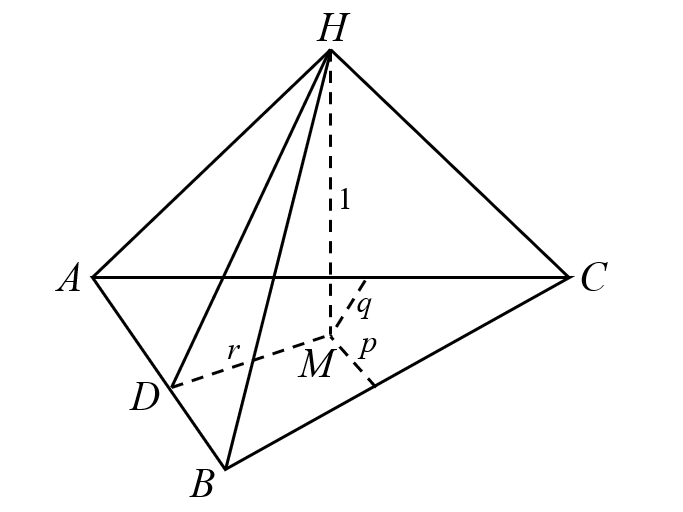
\includegraphics[width=0.35\textwidth]{22B9.png}
    \caption{例\ref{ex:ch06-26}解题用图}
\end{figure}

(3)~~用拉格朗日乘数法.
令$F(p,q,r,\lambda) = S(p,q,r) + \lambda \phi(p,q,r)$.
先求$S$和$\phi$对$p$，$q$，$r$的偏导数：
$$
S_p = \frac{\sqrt{13}}{2} p (1+p^2)^{-\frac{1}{2}}~~~，~~~
S_q = \frac{3\sqrt{5}}{2} q (1+q^2)^{-\frac{1}{2}}~~~，~~~
S_r = \sqrt{10} ~r (1+r^2)^{-\frac{1}{2}}
$$
$$
\phi_p = \sqrt{13}~~，~~
\phi_q = 3\sqrt{5}~~，~~
\phi_r = 2\sqrt{10}
$$\par

列出方程组：

\[
\begin{cases}
    S_p + \lambda \phi_p = \frac{\sqrt{13}}{2} p (1+p^2)^{-\frac{1}{2}} + \sqrt{13} \lambda= 0 \\
    S_q + \lambda \phi_q = \frac{3\sqrt{5}}{2} q (1+q^2)^{-\frac{1}{2}} + 3\sqrt{5} \lambda= 0 \\
    S_r + \lambda \phi_r = \sqrt{10} ~r (1+r^2)^{-\frac{1}{2}}  + 2\sqrt{10} \lambda = 0 \\
    \phi = \sqrt{13} \cdot p + 3\sqrt{5} \cdot q + 2\sqrt{10}\cdot r - 6\sqrt{14} = 0
\end{cases}
\]

由方程组的前三条方程可得：
$$
-2\lambda = \frac{p}{\sqrt{1+p^2}}
= \frac{q}{\sqrt{1+q^2}}
=\frac{r}{\sqrt{1+r^2}}
$$\par
注意到函数$f(x) = \frac{x}{\sqrt{1+x^2}}$在$(0,+\infty)$单调递增，因此上式可以推出$p=q=r$.
代入方程组的第四条方程，解得：
$$
p = q = r = \frac{6\sqrt{14}}{\sqrt{13} + 3\sqrt{5} + 2\sqrt{10}}
$$\par
因此，$S(p,q,r)$在约束条件下的唯一稳定点是：
$$
\left(\frac{6\sqrt{14}}{\sqrt{13} + 3\sqrt{5} + 2\sqrt{10}},~\frac{6\sqrt{14}}{\sqrt{13} + 3\sqrt{5} + 2\sqrt{10}},~\frac{6\sqrt{14}}{\sqrt{13} + 3\sqrt{5} + 2\sqrt{10}}\right)
$$
\end{solution}

\begin{example}[2021]
\label{ex:ch06-27}
给定正整数$n \ge 3$.
求出半径为$1$的圆的内接$n$边形所能达到的最大面积.
\end{example}

\begin{analysis}
根据直觉，当$n$边形为正$n$边形时能达到最大面积.
由于多边形中的变量很多，又受到单位圆的约束，因此拉格朗日乘数法可能是我们的关键手段.
这要求我们尽量简洁地写出面积函数和约束条件.
这里可以设各边所对的圆周角为自变量.

若直接使用拉格朗日乘数法，可以解到稳定点就是正$n$边形时的情况.
但是这不足以说明正$n$边形的面积就是最大，因为还没有讨论边界的情况.
在这个问题中，边界情况就是指$n$边形某条边所对的圆周角为$0$，从而退化成$n-1$边形的情形.
可见，为了严谨地讨论$n$边形的最大面积，不得不连着$n-1$边形一起考虑.
所以，要使用数学归纳法.

\setstretch{2}
\end{analysis}

\begin{solution}
正整数$n \ge 3$时，半径为$1$的圆内接$n$边形（记为$K_n$）所能达到的最大面积是
$\frac{n}{2} \sin \frac{2\pi}{n}$，此时$K_n$为正$n$边形.
接下来证明这个结论.\par

设$K_n$的$n$条边对应的圆心角为$x_1$、$x_2$、$\cdots$、$x_n$，
它们满足约束条件$x_1 + x_2 + \cdots + x_n = 2\pi$.
其中$x_k \ge 0$.
则$K_n$的面积$S_n = \frac{1}{2}\sin x_1 + \frac{1}{2}\sin x_2 + \cdots + \frac{1}{2}\sin x_n$.
我们要证的结论可以翻译成：在约束条件下，$S_n$达到最大值的点是$x_1 = x_2 = \cdots = x_n = \frac{2\pi}{n}$.
最大值为$\frac{n}{2} \sin \frac{2\pi}{n}$.
\par
用数学归纳法证明这个结论.\par
i）先证$n=3$时结论正确.
构造拉格朗日函数：$F(x_1,x_2,x_3,\lambda) = S_n + \lambda (x_1 + x_2 + x_3 -2\pi)$.
然后令：
\[
\begin{cases}
    \frac{\partial F}{\partial x_1} = \frac{1}{2} \cos x_1 + \lambda =0 \\
    \frac{\partial F}{\partial x_2} = \frac{1}{2} \cos x_2 + \lambda =0\\
    \frac{\partial F}{\partial x_3} = \frac{1}{2} \cos x_3 + \lambda =0
\end{cases}
\]\par
解得$x_1 = x_2 = x_3 = \frac{2\pi}{3}$.
这就是区域内部的稳定点.
此时$S_3 = \frac{3}{2} \sin \frac{2\pi}{3}$.
而在区域边界，即$x_1$、$x_2$和$x_3$其中之一等于$0$的情形，
三角形退化为“二边形”，其面积显然为$0$，不可能是最大值.
但是由问题的几何意义，在约束条件所规定的区域上，面积的最大值显然是存在的.
因此可以说明$n=3$时结论正确.\par
ii）假设$n=k$时结论正确，现在证明$n=k+1$时也正确.\par
构造拉格朗日函数：$F(x_1,x_2,\cdot ~x_k,x_{k+1},\lambda) = S_{k+1} + \lambda (x_1+x_2+\cdots + x_k + x_{k+1} - 2\pi)$.
然后令$\frac{\partial F}{\partial x_i}=0$对任意的$1 \le i \le k+1$成立.
即：
$$
\frac{\partial F}{\partial x_i}= \frac{1}{2}\cos x_i + \lambda = 0
$$\par
解得$x_1 = x_2 =\cdot = x_k = x_{k+1} = \frac{2\pi}{k+1}$.
这就是区域内部的稳定点.
此时$S_{k+1} = \frac{k+1}{2} \sin \frac{2\pi}{k+1}$.\par
再考虑区域边界的情况，即$x_1$、$x_2\cdots $$x_{k+1}$其中之一等于$0$的情形.
此时$k+1$边形退化成了$k$边形.
由归纳假设，在区域边界上$S_{k+1}$的最大值（实际上也就是$k$边形面积的最大值）
为$\frac{k}{2}\sin \frac{2\pi}{k}$.
因此，需要证明如下的不等式对$k\ge 3$：
$$
\frac{k}{2}\sin \frac{2\pi}{k} < \frac{k+1}{2}\sin \frac{2\pi}{k+1}
$$\par
只需证明函数$f(x) = \frac{x}{2} \sin \frac{2\pi}{x}$在$x>0$时单调递增.
计算导数并进行放缩：
\begin{equation}
    \begin{aligned}
        f'(x) &= \frac{1}{2} \sin \frac{2\pi}{x} - \frac{\pi}{x} \cos \frac{2\pi}{x} \\
        &= \frac{1}{2}\cos \frac{2\pi}{x} \left( \tan \frac{2\pi}{x} - \frac{2\pi}{x} \right) \\
        &> 0
        \nonumber
    \end{aligned}
\end{equation} \par
这样就证明了$S_{k+1}$不可能是在区域边界上取到最大值.
但是由问题的几何意义，在约束条件所规定的区域上，面积的最大值是存在的.
因此可以说明$n=k+1$时结论正确.\par
综合i）和ii），命题得证.
\end{solution}
